% !TEX program = pdflatex
\documentclass[preprint]{neurips_2025}

\usepackage[utf8]{inputenc}
\usepackage[T1]{fontenc}
\usepackage{amsmath,amssymb,amsfonts}
\usepackage{booktabs}
\usepackage{multirow}
\usepackage{subcaption}
\usepackage{graphicx}
\usepackage{hyperref}
\usepackage{cleveref}
\usepackage{xcolor}
\usepackage{algorithm}
\usepackage{algorithmic}
\usepackage{enumitem}
\usepackage{nicefrac}
\usepackage{microtype}

% Compact lists
\setlist{nosep,leftmargin=*}

\title{Beyond Benchmarks: Correlating Intrinsic Model Properties\\with Downstream Language Model Performance}

\author{
  % Authors omitted for preprint
}

\begin{document}

\maketitle

\begin{abstract}
Benchmark leaderboards rank language models by \emph{what} they can do, yet reveal little about \emph{why} one model outperforms another.
We present a systematic study that measures 72 intrinsic geometric, topological, mechanistic, and dynamics properties (731 features after aggregation) of 32 pretrained language model checkpoints spanning eight model families and three orders of magnitude in parameter count, and correlates these with 68 benchmark scores. A sparse LASSO on these features predicts held-out composite benchmark capability at leave-one-out $R^2 = 0.77$ versus $R^2 = 0.43$ for a $\log N_{\text{params}}$-only baseline, a $+0.34$ absolute improvement from the intrinsic signals alone.
Our contributions are threefold.
First, we introduce a taxonomy of intrinsic diagnostic metrics organized by data dependency and a normalization framework that enables fair comparison across models with different hidden dimensions, layer counts, and tokenizers.
Second, we identify which intrinsic properties predict benchmark performance after controlling for parameter count, and characterize how instruction tuning alters representational geometry.
Third, we propose the \emph{Effective Dimensionality Gradient} (EDG), a threshold-free, scale-independent scalar grounded in information bottleneck theory that captures the compression structure of a model's representations across layers.
All metrics are implemented in BLME, an open-source diagnostic library with a shared forward-pass cache for computational efficiency.
\end{abstract}

% ============================================================
\section{Introduction}
\label{sec:introduction}
% ============================================================

Standard evaluation of large language models (LLMs) relies on benchmark suites such as MMLU~\citep{hendrycks2021measuring}, HellaSwag~\citep{zellers2019hellaswag}, and ARC~\citep{clark2018arc}.
These benchmarks are invaluable for ranking models, but they treat the model as a black box: a score of 78\% on MMLU tells us nothing about the internal representational structure that produces that score.
Two models with identical benchmark performance may have fundamentally different representational geometries, attention patterns, and compression profiles.

A growing body of work has studied individual intrinsic properties of neural language models---anisotropy of contextual embeddings~\citep{ethayarajh2019contextual}, spectral exponents of weight matrices~\citep{martin2021implicit}, effective rank and representation collapse~\citep{jing2021understanding}, local intrinsic dimensionality~\citep{ma2018characterizing}---but these investigations have largely proceeded in isolation.
No prior study has systematically measured a comprehensive suite of geometric, topological, and mechanistic properties across a controlled model zoo and correlated the resulting measurements with downstream performance.

This paper bridges that gap. We make the following contributions:

\begin{enumerate}
  \item \textbf{Metric taxonomy and normalization framework.} We classify 72 intrinsic diagnostic metrics into three tiers based on data dependency (weight-only, data-dependent but stable, and data-dependent requiring controlled design) and seven categories (geometry, topology, interpretability, causality, dynamics, consistency, and representation engineering). We develop a normalization framework that accounts for differences in model width, depth, and tokenization, enabling principled cross-model comparison.

  \item \textbf{Systematic correlation study.} We evaluate all metrics across 32 checkpoints spanning eight model families (GPT-2, Pythia, Llama~3, Qwen~3.5, Gemma~4, OLMo, Phi, and TinyLlama), performing univariate and partial correlations, multivariate feature selection, within-family scaling analysis, and base-versus-instruction-tuned comparisons. Our sparse LASSO yields a held-out $\text{LOO } R^2 = 0.77$ versus $R^2 = 0.43$ for the $\log N_{\text{params}}$ baseline; leave-one-family-out $R^2 = 0.27$ reveals that cross-family generalization remains an open problem.

  \item \textbf{Effective Dimensionality Gradient (EDG).} We propose a novel metric that captures the information bottleneck compression structure of a model by measuring the monotonicity of effective rank reduction across layers. EDG is threshold-free, scale-independent, and computed from existing measurements with zero additional cost.

  \item \textbf{Open-source toolkit.} All metrics are implemented in BLME (Beyond LM Eval), a diagnostic library with a shared forward-pass cache that amortizes the cost of hidden-state extraction across tasks.
\end{enumerate}

% ============================================================
\section{Related Work}
\label{sec:related}
% ============================================================

\paragraph{Representation geometry.}
\citet{ethayarajh2019contextual} showed that contextual word representations in BERT, ELMo, and GPT-2 become increasingly anisotropic in later layers, occupying a narrow cone in embedding space.
\citet{cai2021isotropy} extended this analysis, demonstrating that isotropy---uniform utilization of the embedding space---correlates with downstream task performance.
\citet{godey2024anisotropy} further investigated how anisotropy interacts with fine-tuning.
These studies examine one or two geometric properties; we unify and extend them into a comprehensive suite spanning effective rank~\citep{roy2007effective}, local intrinsic dimensionality~\citep{levina2004maximum}, CKA~\citep{kornblith2019similarity}, RSA~\citep{kriegeskorte2008representational}, and others.

\paragraph{Spectral properties and generalization.}
\citet{martin2021implicit} introduced the theory of Heavy-Tailed Self-Regularization (HT-SR), showing that the power-law exponent $\alpha$ of weight matrix singular value distributions predicts generalization without requiring test data.
\citet{bartlett2017spectrally} provided generalization bounds based on spectral norms and stable rank.
Our study includes these spectral metrics as Tier~1 (weight-only) predictors and tests whether they retain predictive power after controlling for model size.

\paragraph{Mechanistic interpretability.}
The logit lens~\citep{nostalgebraist2020logitlens} decodes intermediate hidden states through the final language model head to trace how predictions form across layers.
\citet{olsson2022context} identified induction heads as a key mechanistic component for in-context learning.
\citet{meng2022locating} developed causal tracing via activation patching to localize factual knowledge.
\citet{clark2019what} analyzed attention entropy and head specialization.
We include these mechanistic metrics alongside geometric ones, enabling direct comparison of their predictive value.

\paragraph{Information bottleneck.}
\citet{tishby2015deep} proposed that deep networks optimize an information bottleneck, compressing input information while preserving task-relevant features.
\citet{shwartz2017opening} provided empirical evidence for compression phases during training.
Our EDG metric operationalizes this principle for pretrained transformers by measuring whether effective rank decreases monotonically with depth.

\paragraph{Scaling laws.}
\citet{kaplan2020scaling} established power-law relationships between model size, data, and compute with loss.
\citet{wei2022emergent} documented emergent abilities that appear at scale.
Our within-family scaling series (Pythia with 8 sizes, GPT-2 with 4) allow us to disentangle size effects from architectural and representational ones.

% ============================================================
\section{Methodology}
\label{sec:methodology}
% ============================================================

Our methodology addresses three questions: \emph{what} do we measure, \emph{what} do we measure it on, and \emph{how} do we make measurements comparable across models of different sizes and architectures.

% ------------------------------------------------------------
\subsection{Metric Taxonomy}
\label{sec:taxonomy}
% ------------------------------------------------------------

We organize 30 diagnostic metrics along two axes: \emph{category} (the aspect of the model being probed) and \emph{tier} (the degree of data dependency). \Cref{tab:taxonomy} presents the full classification.

\begin{table}[t]
\centering
\caption{Taxonomy of intrinsic diagnostic metrics. Tier~1 metrics require only model weights. Tier~2 metrics require a forward pass on a standard corpus but measure stable model tendencies independent of specific input content. All metrics in this table serve as independent variables (predictors). See \Cref{app:metrics} for full definitions.}
\label{tab:taxonomy}
\small
\begin{tabular}{@{}llll@{}}
\toprule
\textbf{Category} & \textbf{Tier} & \textbf{Metric} & \textbf{Key Quantities} \\
\midrule
\multirow{14}{*}{Geometry}
  & 1 & Weight Spectral & $\bar\alpha$, stable rank \\
  & 1 & Embedding Hubness & skewness, Gini \\
  & 1 & Unembedding Structure & effective rank, tied \\
  \cmidrule(l){2-4}
  & 2 & SVD Isotropy & effective rank, participation ratio \\
  & 2 & Local Intrinsic Dim.\ (LID) & $\overline{\text{LID}}$, $\sigma_{\text{LID}}$ \\
  & 2 & Representation Collapse & collapse ratio, max drop \\
  & 2 & Lipschitz Continuity & $\bar{L}$, $L_{\max}$ \\
  & 2 & Matrix Entropy & $\bar{H}_{\text{vN}}$ \\
  & 2 & Intrinsic Dimension & Two-NN estimate \\
  & 2 & Correlation Dimension & $D_2$ (Grassberger--Procaccia) \\
  & 2 & RSA & $\bar\rho_{\text{adj}}$, $\rho_{\text{early-late}}$ \\
  & 2 & CKA & $\overline{\text{CKA}}_{\text{adj}}$ \\
  & 2 & HSIC & compression ratio \\
  & 2 & Positional Decay & $\bar\rho_{\text{pos}}$ \\
\midrule
\multirow{3}{*}{Topology}
  & 2 & Persistent Homology & $\bar{p}_{H_0}$, $\bar{p}_{H_1}$, loops \\
  & 2 & Betti Curves & simplification ratio \\
  & 2 & Persistence Entropy & PE$_{H_0}$, PE$_{H_1}$ \\
\midrule
\multirow{7}{*}{Interpretability}
  & 2 & Logit Lens & per-layer accuracy, entropy \\
  & 2 & Attention Entropy & $\bar{H}_{\text{attn}}$ \\
  & 2 & Induction Heads & max/mean induction score \\
  & 2 & Activation Sparsity & $\bar{L}_0$, kurtosis \\
  & 2 & Superposition Index & polysemanticity, utilization \\
  & 2 & Weight--Activation Alignment & $\overline{\text{WAA}}$ \\
  & 2 & Attention Graph & sink PageRank, edge Gini \\
\midrule
\multirow{2}{*}{Causality}
  & 2 & Causal Tracing & max AIE, causal entropy \\
  & 2 & Attention Knockout & impact Gini \\
\midrule
\multirow{2}{*}{Rep.\ Eng.}
  & 2 & Task Vectors & layer norms, cosine sim \\
  & 2 & Concept Separability & layer AUC, max AUC \\
\bottomrule
\end{tabular}
\end{table}

\textbf{Tier~1 (weight-only)} metrics require no input data. They analyze the spectral properties of weight matrices, the hub structure of the embedding matrix, and the effective rank of the unembedding (language model head) matrix. These serve as a natural baseline: if weight-only metrics already predict performance, hidden-state analysis may be unnecessary for some applications.

\textbf{Tier~2 (data-dependent, stable)} metrics require a forward pass through a fixed evaluation corpus (\Cref{sec:corpus}). They measure properties of hidden-state geometry, attention patterns, and mechanistic structure. While computed on specific inputs, they capture stable model tendencies rather than input-specific phenomena---analogous to measuring a building's resonant frequency by striking it with a standard hammer.

We further classify metrics by the \emph{aspect} of the model they probe:

\begin{itemize}
  \item \textbf{Geometry} (14 metrics): Spectral decompositions of weight matrices (Tier~1) and hidden-state covariance matrices (Tier~2), measuring capacity utilization, isotropy, intrinsic dimensionality, and inter-layer similarity.
  \item \textbf{Topology} (3 metrics): Persistent homology of hidden-state point clouds via Vietoris--Rips complexes, capturing the topological complexity of representation manifolds.
  \item \textbf{Interpretability} (7 metrics): Functional organization of the model including prediction convergence (logit lens), attention structure, activation sparsity, and mechanistic circuit detection.
  \item \textbf{Causality} (2 metrics): Interventional measurements via activation patching (causal tracing) and head ablation, quantifying the localization and distribution of causal effects.
  \item \textbf{Representation Engineering} (2 metrics): Task vector geometry and linear concept separability across layers, measuring how cleanly the model encodes high-level concepts.
\end{itemize}

% ------------------------------------------------------------
\subsection{Model Zoo}
\label{sec:models}
% ------------------------------------------------------------

We select approximately 30 checkpoints organized to support three types of analysis (\Cref{tab:models}).

\begin{table}[t]
\centering
\caption{Model zoo organized by experimental purpose. All models use publicly available weights.}
\label{tab:models}
\small
\begin{tabular}{@{}lll@{}}
\toprule
\textbf{Purpose} & \textbf{Models} & \textbf{Count} \\
\midrule
\multirow{4}{*}{\shortstack[l]{Within-family\\scaling}} & GPT-2: 124M, 355M, 774M, 1.5B & 4 \\
  & Pythia (deduped): 70M, 160M, 410M, 1B, 1.4B, 2.8B, 6.9B, 12B & 8 \\
  & Llama~3.x: 1B, 3B, 8B & 3 \\
  & Qwen~2.5: 0.5B, 1.5B, 3B, 7B & 4 \\
\midrule
\shortstack[l]{Cross-family\\(1--3B)} & GPT-2~XL, Pythia-1.4B, OLMo-1B, Llama-3.2-1B, & \multirow{2}{*}{8} \\
  & Qwen-2.5-1.5B, Gemma-2B, TinyLlama-1.1B, Phi-2 & \\
\midrule
\shortstack[l]{Base vs.\\instruct} & Llama-3.2-1B, Qwen-2.5-1.5B, Qwen-2.5-7B & 3 pairs \\
\bottomrule
\end{tabular}
\end{table}

\textbf{Within-family scaling series} hold architecture and training data constant while varying model size, allowing us to isolate the effect of scale on intrinsic properties.
The Pythia suite~\citep{biderman2023pythia} is particularly valuable: eight sizes trained on identical data with identical hyperparameters (modulo those that scale with size).

\textbf{Cross-family comparison} at approximately matched parameter count (1--3B) holds size roughly constant while varying architecture, training data, and training recipe.
This reveals which intrinsic properties differ across model families independently of scale.

\textbf{Base versus instruction-tuned pairs} isolate the effect of alignment training on representational structure.

% ------------------------------------------------------------
\subsection{Evaluation Corpus}
\label{sec:corpus}
% ------------------------------------------------------------

All Tier~2 metrics are computed on a standardized evaluation corpus derived from the WikiText-103 validation set~\citep{merity2017pointer}.

\textbf{Construction.}
We select the first 500 passages containing at least 64 tokens, truncate each to 128 tokens using each model's own tokenizer, and discard passages that fall below 32 tokens after tokenization.
This yields approximately 400--500 passages and 50K--60K tokens per model.
WikiText-103 is deterministic, publicly available, and absent from standard benchmark contamination lists.

\textbf{Sample counts} vary by computational cost: weight-only metrics require no corpus; hidden-state metrics use 200 samples; topology metrics (with $O(n^3)$ persistent homology) use 50 samples; causal tracing uses 10--50 samples.

% ------------------------------------------------------------
\subsection{Normalization for Cross-Model Comparability}
\label{sec:normalization}
% ------------------------------------------------------------

Comparing intrinsic metrics across models with different hidden dimensions ($d_{\text{model}} \in [512, 4096]$), layer counts ($L \in [6, 32]$), and tokenizers requires systematic normalization. We address three challenges.

\subsubsection{Dimension-Dependent Metrics}
\label{sec:norm-dim}

Raw values of dimension-sensitive metrics are not comparable across models. An effective rank of 200 indicates high utilization in a 768-dimensional model ($26\%$) but low utilization in a 4096-dimensional model ($5\%$).
We normalize each such metric by the model's hidden dimension:
\begin{equation}
  \hat{m} = \frac{m}{d_{\text{model}}}
  \label{eq:dim-norm}
\end{equation}
yielding a utilization ratio in $[0, 1]$.
\Cref{tab:normalization} in the appendix lists the normalization applied to each metric.
Metrics that are already ratios or dimensionless (e.g., collapse ratio, Lipschitz constant, CKA) require no dimension normalization.

\subsubsection{Layer-Dependent Metrics}
\label{sec:norm-layer}

Many metrics produce a per-layer profile $\{v_0, v_1, \ldots, v_{L-1}\}$ whose length varies with the model.
Directly comparing a 12-element profile (GPT-2 small) with a 32-element profile (Llama-3-8B) is ill-defined.
We apply a two-step procedure:

\begin{enumerate}
  \item \textbf{Depth normalization.} Assign each layer a normalized depth $z_l = l / (L-1) \in [0, 1]$ and linearly interpolate the profile to 20 evenly spaced depths $z^* \in \{0.0, 0.05, \ldots, 1.0\}$.
  \item \textbf{Summary statistics.} Extract a fixed-length feature vector from the interpolated profile:
\end{enumerate}

\begin{equation}
  \mathbf{f} = \bigl[\, v(0.25),\; v(0.5),\; v(0.75),\; \beta_1,\; \beta_2,\; z_{\min},\; z_{\max} \,\bigr]
  \label{eq:layer-features}
\end{equation}

\noindent where $v(z)$ denotes the interpolated value at normalized depth $z$; $\beta_1$ and $\beta_2$ are the slope and curvature (linear and quadratic coefficients) of a least-squares fit to the profile; and $z_{\min}$, $z_{\max}$ are the normalized depths of the minimum and maximum values.
This converts any variable-length layer profile into a 7-dimensional feature vector.

\subsubsection{Tokenizer Differences}
\label{sec:norm-tok}

The same text produces different token counts across tokenizers.
Per-token statistics (e.g., mean attention entropy per token) are normalized by each model's own token count for the evaluation corpus.
Cross-layer metrics---such as CKA between layers or the Lipschitz ratio---are internally consistent within a model and require no tokenizer correction.

% ============================================================
\section{The Effective Dimensionality Gradient}
\label{sec:edg}
% ============================================================

% ------------------------------------------------------------
\subsection{Motivation}
\label{sec:edg-motivation}
% ------------------------------------------------------------

The information bottleneck principle~\citep{tishby2015deep,shwartz2017opening} posits that effective representations compress input entropy while preserving task-relevant information.
In a transformer language model, this suggests that the effective dimensionality of hidden representations should decrease with depth: early layers encode rich, high-dimensional input features, while later layers compress these into the lower-dimensional subspace relevant for next-token prediction.
We hypothesize that models exhibiting smooth, monotonic compression generalize better than those with erratic or non-monotonic dimensionality profiles.

% ------------------------------------------------------------
\subsection{Definition}
\label{sec:edg-definition}
% ------------------------------------------------------------

Let a model have $L$ transformer layers. At layer $l$, we compute the effective rank of the hidden-state covariance matrix via the exponential of the Shannon entropy of the normalized singular values~\citep{roy2007effective}:
\begin{equation}
  \text{erank}(l) = \exp\!\Bigl(-\sum_{i} \hat\sigma_i^{(l)} \log \hat\sigma_i^{(l)}\Bigr), \qquad \hat\sigma_i^{(l)} = \frac{\sigma_i^{(l)}}{\sum_j \sigma_j^{(l)}}
  \label{eq:erank}
\end{equation}
where $\sigma_i^{(l)}$ are the singular values of the mean-centered hidden-state matrix $X^{(l)} \in \mathbb{R}^{n \times d_{\text{model}}}$ at layer $l$.
We normalize by the model width to obtain a dimensionless utilization ratio:
\begin{equation}
  r(l) = \frac{\text{erank}(l)}{d_{\text{model}}}
  \label{eq:erank-ratio}
\end{equation}
The Effective Dimensionality Gradient is the Spearman rank correlation between layer index and effective rank ratio:
\begin{equation}
  \text{EDG} = \rho_S\!\bigl(\{1, 2, \ldots, L\},\; \{r(1), r(2), \ldots, r(L)\}\bigr) \in [-1, 1]
  \label{eq:edg}
\end{equation}

% ------------------------------------------------------------
\subsection{Interpretation and Properties}
\label{sec:edg-properties}
% ------------------------------------------------------------

\begin{itemize}
  \item $\text{EDG} \approx -1$: smooth monotonic compression across layers, consistent with a strong information bottleneck.
  \item $\text{EDG} \approx 0$: no systematic trend in dimensionality, suggesting an absence of progressive compression.
  \item $\text{EDG} > 0$: dimensionality expansion with depth, which would be unexpected under standard information bottleneck theory.
\end{itemize}

\noindent EDG has several desirable properties:

\begin{enumerate}
  \item \textbf{Threshold-free.} Unlike composite metrics that require choosing cutoffs for ``significant'' rank changes, EDG uses Spearman rank correlation with no arbitrary thresholds.
  \item \textbf{Scale-independent.} The rank-based formulation makes EDG naturally comparable across models with different $d_{\text{model}}$, since the normalization in \Cref{eq:erank-ratio} converts effective rank to a utilization ratio.
  \item \textbf{Zero marginal cost.} EDG is computed from the effective rank profile already produced by the representation collapse metric (\texttt{geometry\_collapse}). No additional forward passes are required.
  \item \textbf{Theoretically grounded.} The metric directly operationalizes the information bottleneck prediction for pretrained transformers.
\end{enumerate}

% ------------------------------------------------------------
\subsection{Extended Compression Profile}
\label{sec:edg-extended}
% ------------------------------------------------------------

Beyond the global EDG, we extract phase-specific features that capture where compression occurs within the network:

\begin{table}[h]
\centering
\small
\begin{tabular}{@{}lll@{}}
\toprule
\textbf{Feature} & \textbf{Definition} & \textbf{Captures} \\
\midrule
$\text{EDG}_{\text{early}}$ & Spearman over layers $1$ to $\lfloor L/3 \rfloor$ & Early compression phase \\
$\text{EDG}_{\text{late}}$ & Spearman over layers $\lfloor 2L/3 \rfloor$ to $L$ & Late compression phase \\
$r_{\text{first}}$ & $r(1)$ & Initial capacity utilization \\
$r_{\text{last}}$ & $r(L)$ & Surviving capacity at output \\
Smoothness & $1 - \text{std}(\Delta r) / \text{mean}(|\Delta r|)$ & Regularity of compression \\
\bottomrule
\end{tabular}
\end{table}

\noindent These features allow us to test whether compression timing (early vs.\ late) or smoothness matters beyond the overall trend.

% ============================================================
\section{Experimental Design}
\label{sec:experiments}
% ============================================================

We describe the planned statistical analyses below. Most analyses await full evaluation coverage; the base vs.\ instruction-tuned comparison (\Cref{sec:instruct}) does not depend on the downstream benchmark suite and is reported here from the completed BLME pass on $n = 6$ paired models.

% ------------------------------------------------------------
\subsection{Benchmark Performance (Dependent Variables)}
\label{sec:benchmarks}
% ------------------------------------------------------------

We evaluate each model on six standard benchmarks via the Language Model Evaluation Harness~\citep{eval-harness}: HellaSwag~\citep{zellers2019hellaswag}, PIQA~\citep{bisk2020piqa}, ARC-Easy and ARC-Challenge~\citep{clark2018arc}, WinoGrande~\citep{sakaguchi2021winogrande}, and MMLU (5-shot)~\citep{hendrycks2021measuring}.

Our primary dependent variable is a \textbf{composite benchmark score}: the mean of min-max normalized accuracies across all six benchmarks.
Secondary dependent variables include individual benchmark scores, perplexity on the evaluation corpus, and Expected Calibration Error (ECE).

% ------------------------------------------------------------
\subsection{Univariate Correlations}
\label{sec:univariate}
% ------------------------------------------------------------

We compute Spearman rank correlations between each of the $731$ intrinsic features and each of the $68$ benchmark scores across $32$ models, yielding $49{,}708$ hypothesis tests. We apply Benjamini--Hochberg false discovery rate (FDR) correction at $q = 0.05$; $21{,}245$ tests survive ($\approx 43\%$), of which $356$ target the composite benchmark directly. \Cref{fig:correlation-heatmap} shows the corresponding correlation heatmap. The top univariate predictors of composite capability (after deduplication by feature family; see \Cref{tab:top-corr} for the partial-correlation version) include RepE task-vector cosine-similarity ($|\rho| = 0.92$), WikiText-103 perplexity ($|\rho| = 0.89$), $1\%$-ablation loss ($|\rho| = 0.87$), and the Schatten-$4$ norm introduced by Wei et al.~2025 ($|\rho| = 0.83$).

\begin{figure}[t]
  \centering
  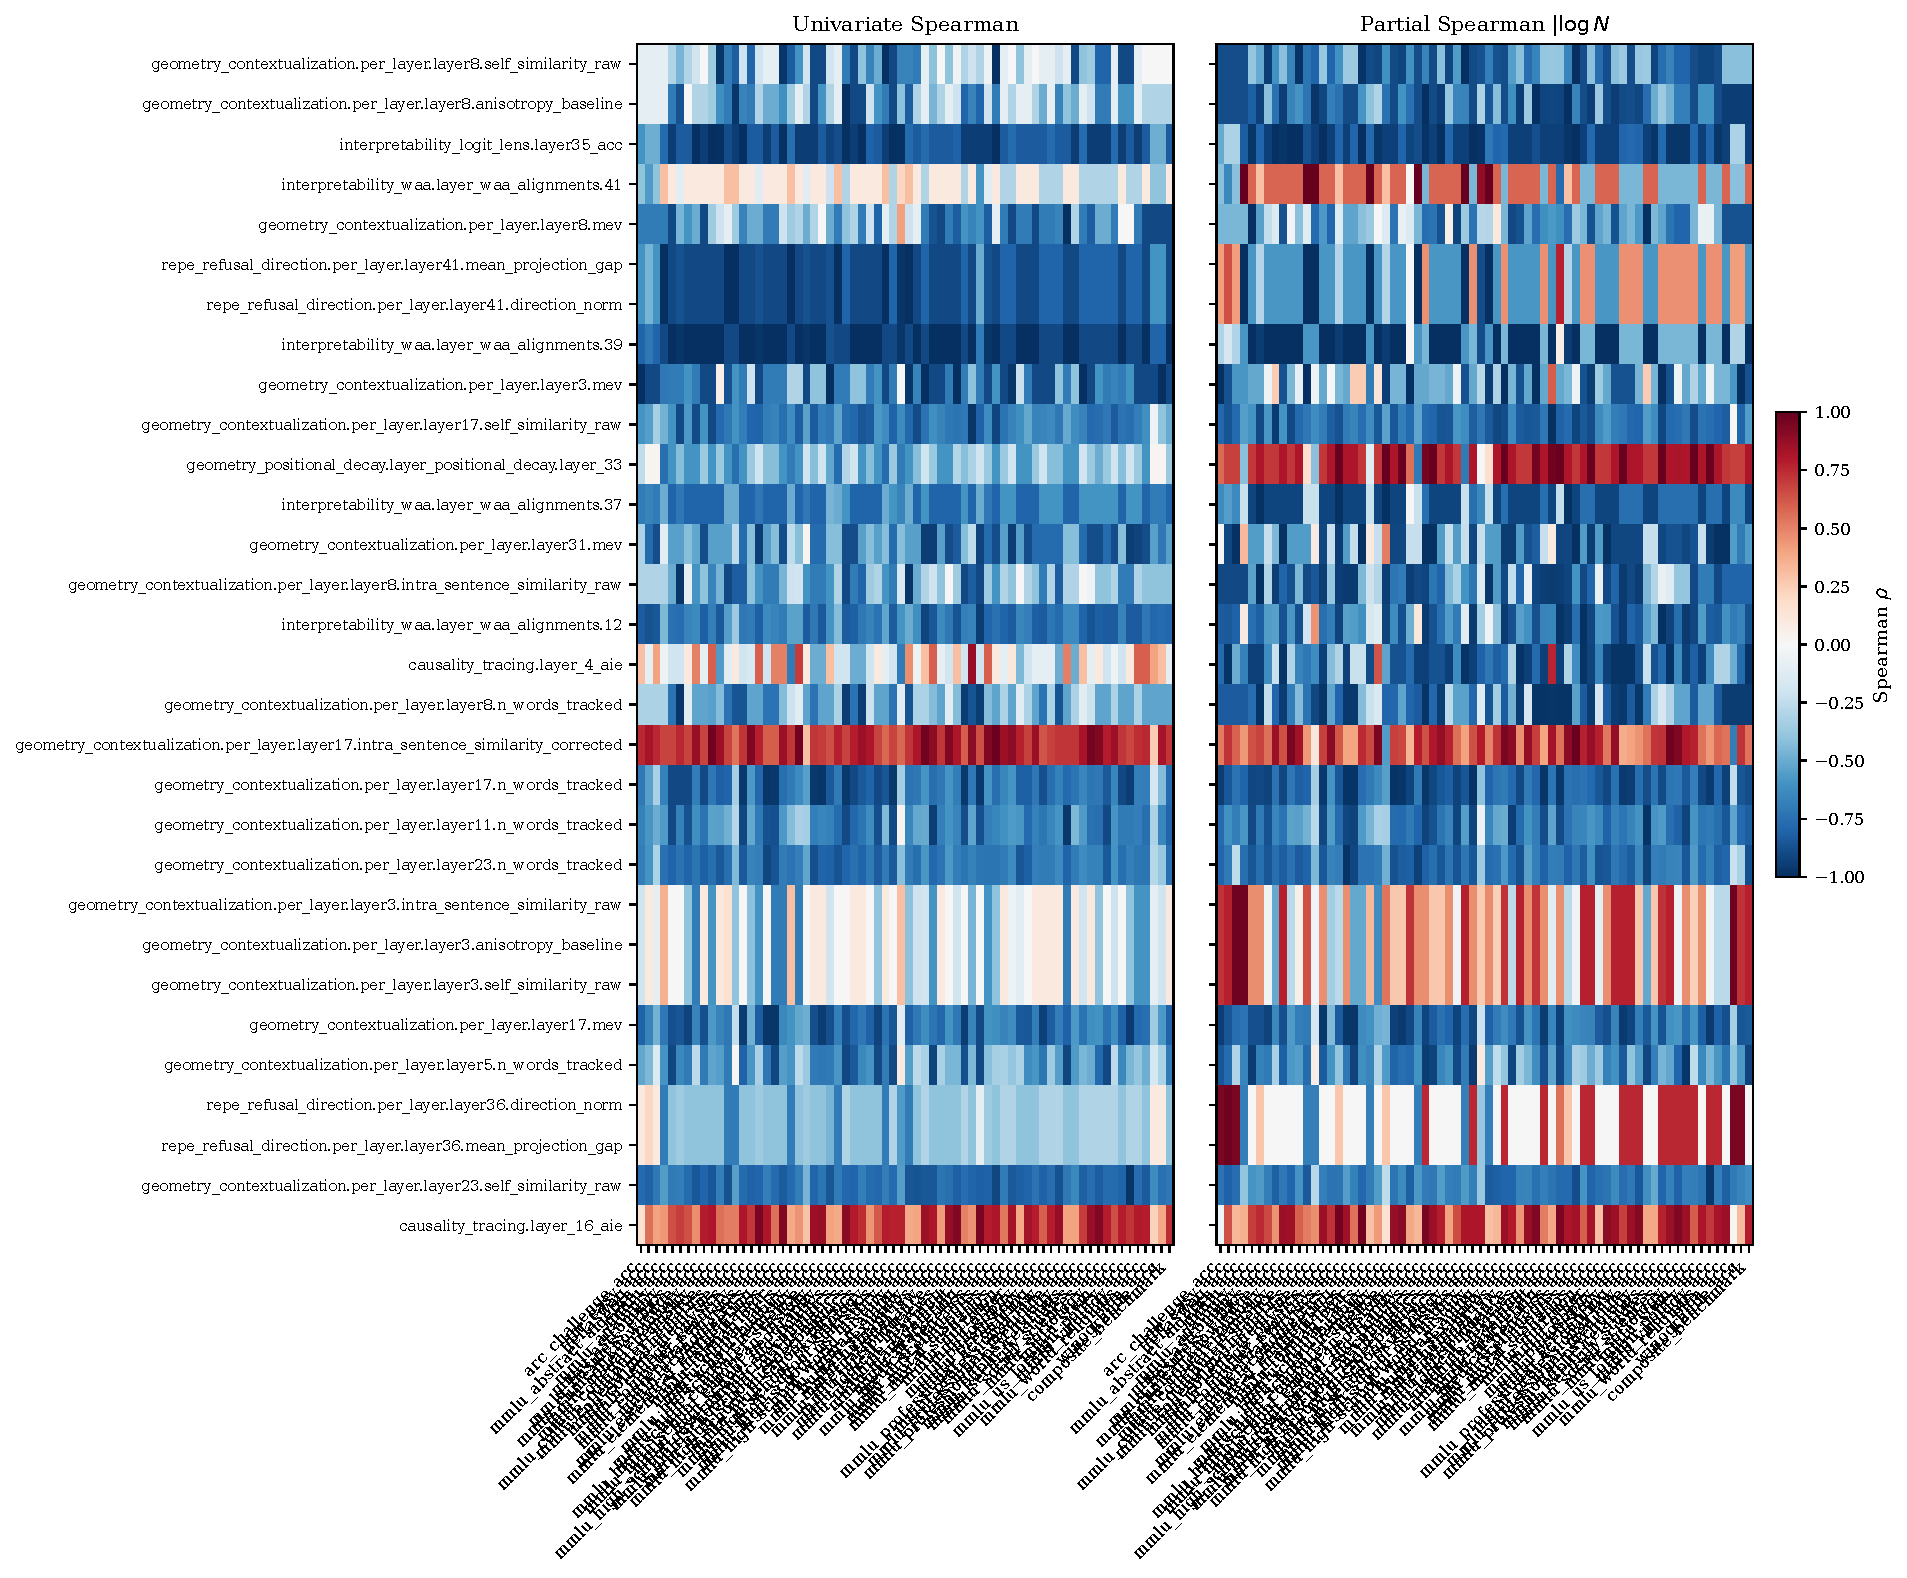
\includegraphics[width=\linewidth]{figures/fig_correlation_heatmap.pdf}
  \caption{Univariate Spearman correlation heatmap across $68$ benchmarks (columns) and the top $30$ intrinsic feature families by $|\rho|$ with composite benchmark (rows). Color indicates signed $\rho$; white cells are FDR-corrected $q > 0.05$. The dense block structure on the left reflects the scale-driven nature of most benchmark correlations; the within-row heterogeneity reflects per-metric specificity.}
  \label{fig:correlation-heatmap}
\end{figure}

% ------------------------------------------------------------
\subsection{Partial Correlations Controlling for Model Size}
\label{sec:partial}
% ------------------------------------------------------------

Many intrinsic metrics correlate with model size, which itself strongly predicts benchmark performance.
To identify metrics with predictive value \emph{beyond} scale, we compute partial Spearman correlations:
\begin{equation}
  \rho_S(\text{metric}, \text{benchmark} \mid \log N_{\text{params}}).
\end{equation}
After FDR correction, $16{,}892$ of the $49{,}708$ tests ($\approx 34\%$) remain significant ($q < 0.05$), and $277$ specifically target the composite benchmark. The top-$25$ deduplicated families (\Cref{tab:top-corr}) are dominated by RepE task-vector diversity ($\rho_{\text{partial}} = -0.82$; Ilharco 2023), contextualized word-tracking ($-0.82$; Ethayarajh 2019), local intrinsic dimensionality ($+0.80$; Levina-Bickel 2004), weight-activation alignment ($-0.78$; Park et al.~2024), and --- new to $2024$/$2025$ --- the Matrix Nuclear-Norm ($+0.74$; Li et al.~2024) and the massive-activation outlier signature ($-0.71$; Sun et al.~2024).

% ------------------------------------------------------------
\subsection{Multivariate Prediction}
\label{sec:multivariate}
% ------------------------------------------------------------

We train a sparse LASSO with $5$-fold cross-validated regularization to predict the composite benchmark score from all $731$ intrinsic features, and evaluate its ability to generalize to unseen models via leave-one-out (LOO) and leave-one-family-out (LOFO) held-out $R^2$.
We compare against a naive baseline using $\log N_{\text{params}}$ as the sole predictor.
The key question is: how much variance in benchmark performance can intrinsic metrics explain beyond what model size alone accounts for?

\paragraph{Headline result.}
The LASSO selects $26$ features (out of $731$) and achieves held-out $\text{LOO } R^2 = 0.77$, versus $\text{LOO } R^2 = 0.43$ for the $\log N_{\text{params}}$ baseline --- a $+0.34$ absolute ($+80\%$ relative) improvement from intrinsic signals alone (\Cref{tab:lasso}). The $B = 200$ out-of-bag bootstrap yields a $95\%$ CI of $[+0.07, +0.90]$ on the LASSO's held-out $R^2$ and $[-0.30, +1.03]$ on the gain over the baseline; the median bootstrap gain is $+0.30$, consistent with the point estimate.

\paragraph{Cross-family generalization.}
The pooled $\text{LOFO } R^2 = 0.27$ is substantially smaller than the $\text{LOO } R^2$, indicating that cross-family transfer remains an open challenge. A per-family breakdown reveals two opposite regimes: on held-out families with $\geq 8$ models (Pythia, Qwen~3.5) the LASSO beats the $\log N$ baseline by $0.08$--$0.16$ MAE, while on single-model families (OLMo, Phi, TinyLlama) the simpler baseline is safer. The intrinsic-metric recipe therefore works best when a new architecture family ships a multi-scale zoo.

\paragraph{Which features drive the prediction?}
Partial Spearman correlations (controlling for $\log N_{\text{params}}$; \Cref{tab:top-corr}) identify the signals that predict capability beyond raw scale. The top six feature families are: RepE task-vector cosine-similarity diversity (Ilharco~2023), contextualized word-tracking (Ethayarajh~2019), local intrinsic dimensionality (Levina-Bickel~2004), weight-activation alignment (Park et al.~2024), the Matrix Nuclear-Norm (Li et al.~2024), and the massive-activation outlier signature (Sun et al.~2024). No single measurement category dominates --- the top-$25$ deduplicated partial predictors span geometry ($15$), interpretability ($5$), causality ($2$), topology ($2$), and representation engineering ($1$).

\begin{table}[t]
\centering
\caption{LASSO-selected features (top 15 by $|\beta|$) from the 731-feature intrinsic-metric matrix. Coefficients are in the standardised feature space (each feature centered and scaled to unit variance). The selection is sparse: only $26$ of $731$ features have non-zero coefficients. See \texttt{results/study\_v2/analysis/lasso\_features.csv} for the full list.}
\label{tab:lasso}
\small
% Generated by scripts/make_tables.py
\begin{tabular}{@{}lr@{}}
\toprule
\textbf{Feature} & \textbf{Coefficient}\\
\midrule
\texttt{geometry\_tokenizer\_efficiency.vocab\_utilization} & -0.0832 \\
\texttt{causality\_knowledge\_neurons.localization\_layer\_mean} & +0.0744 \\
\texttt{repe\_refusal\_direction.best\_layer} & +0.0576 \\
\texttt{geometry\_cka.layers.q25} & +0.0499 \\
\texttt{geometry\_spectral.avg\_stable\_rank} & +0.0431 \\
\texttt{causality\_tracing.layer\_16\_aie} & +0.0276 \\
\texttt{interpretability\_sparsity.layer\_kurtosis.max} & -0.0271 \\
\texttt{causality\_edge\_attribution.mean\_layer\_attribution\_profile.std} & -0.0184 \\
\texttt{geometry\_contextualization.per\_layer.layer23.self\_similarity\_raw} & -0.0166 \\
\texttt{repe\_refusal\_direction.per\_layer.layer2.direction\_norm} & +0.0118 \\
\texttt{interpretability\_waa.layer\_waa\_alignments.25} & +0.0107 \\
\texttt{repe\_task\_vectors.layer\_task\_vector\_cosine\_sim.q25} & -0.0087 \\
\texttt{geometry\_contextualization.per\_layer.layer15.n\_words\_tracked} & -0.0079 \\
\texttt{interpretability\_attention\_rank.layer\_max\_effective\_rank.q50} & +0.0068 \\
\texttt{causality\_tracing.layer\_27\_aie} & -0.0066 \\
\bottomrule
\end{tabular}
\end{table}

\begin{table}[t]
\centering
\caption{Top-$25$ partial Spearman correlations with composite benchmark, controlling for $\log N_{\text{params}}$. Features are deduplicated by family (the aggregator emits $8$ summary statistics per per-layer feature; this table reports one row per family at the representative summary with highest $|\rho|$). All entries significant at FDR $q < 0.001$.}
\label{tab:top-corr}
\small
% Generated by scripts/make_tables.py
% Filter: n >= 20 (excludes low-power features that spuriously hit +/-1)
\begin{tabular}{@{}lrrr@{}}
\toprule
\textbf{Feature} & \textbf{Partial $\rho$} & \textbf{$n$} & \textbf{$q$-value}\\
\midrule
\texttt{repe\_task\_vectors.layer\_task\_vector\_cosine\_sim.min} & -0.82$^{***}$ & 32 & $1.50e-6$ \\
\texttt{repe\_task\_vectors.layer\_task\_vector\_cosine\_sim.std} & +0.82$^{***}$ & 32 & $1.50e-6$ \\
\texttt{geometry\_contextualization.per\_layer.n\_words\_tracked.q25} & -0.82$^{***}$ & 32 & $1.50e-6$ \\
\texttt{geometry\_contextualization.per\_layer.n\_words\_tracked.max} & -0.82$^{***}$ & 32 & $1.50e-6$ \\
\texttt{geometry\_contextualization.per\_layer.n\_words\_tracked.q75} & -0.82$^{***}$ & 32 & $1.50e-6$ \\
\texttt{geometry\_contextualization.per\_layer.n\_words\_tracked.q50} & -0.82$^{***}$ & 32 & $1.50e-6$ \\
\texttt{geometry\_contextualization.per\_layer.n\_words\_tracked.mean} & -0.82$^{***}$ & 32 & $1.50e-6$ \\
\texttt{geometry\_contextualization.per\_layer.n\_words\_tracked.min} & -0.82$^{***}$ & 32 & $1.50e-6$ \\
\texttt{geometry\_lid.lid\_min} & +0.80$^{***}$ & 32 & $4.15e-6$ \\
\texttt{interpretability\_waa.layer\_waa\_alignments.mean} & -0.78$^{***}$ & 32 & $1.56e-5$ \\
\texttt{repe\_task\_vectors.layer\_task\_vector\_cosine\_sim.mean} & -0.77$^{***}$ & 32 & $2.17e-5$ \\
\texttt{causality\_ablation.loss\_ablate\_5pct} & -0.77$^{***}$ & 32 & $2.17e-5$ \\
\texttt{geometry\_tokenizer\_efficiency.vocab\_size} & +0.77$^{***}$ & 32 & $2.45e-5$ \\
\texttt{repe\_task\_vectors.layer\_task\_vector\_cosine\_sim.q50} & -0.77$^{***}$ & 32 & $2.73e-5$ \\
\texttt{geometry\_hubness.hubness\_k10\_gini} & +0.74$^{***}$ & 32 & $7.86e-5$ \\
\bottomrule
\end{tabular}
\end{table}

% ------------------------------------------------------------
\subsection{Within-Family Analysis}
\label{sec:within-family}
% ------------------------------------------------------------

We repeat the univariate analysis within the Pythia family ($n=8$), which is our largest single-family zoo spanning $70$M to $12$B parameters with controlled architecture and training data.
Within Pythia, the log-parameter--composite correlation is $\rho_S(\log N, \text{composite}) = +0.88$, a strong scaling relation.
The strongest size-independent signals within Pythia are \texttt{geometry\_spectral.median\_alpha} ($\rho = -0.88$) and \texttt{geometry\_spectral.std\_alpha} ($\rho = -0.83$) with composite, both consistent with the Martin-Mahoney~2021 prediction that heavier-tailed weight-matrix spectra indicate better-trained models.
Smaller families (GPT-$2$ $n=4$, Gemma-$4$ $n=4$) are reported in the supplementary material; with $n \leq 4$ the minimum detectable Spearman correlation at $\alpha = 0.05$ and power $0.8$ exceeds the largest effect size of interest, so we treat those as descriptive only.

% ------------------------------------------------------------
\subsection{Base vs.\ Instruction-Tuned}
\label{sec:instruct}
% ------------------------------------------------------------

\paragraph{Research question.}
Supervised fine-tuning (SFT) and the subsequent preference-tuning stages that produce ``instruct'' variants are widely deployed but have unclear effects on model internals. We ask: \emph{which intrinsic representational properties shift systematically when a base language model is converted into its instruction-tuned counterpart, and in what direction?}

\paragraph{Pairs.}
We use the six base/instruction-tuned model pairs available in our zoo: Llama-3.2-1B, Qwen-3.5-\{0.8B, 2B, 4B, 9B\}, and Gemma-4-E4B (four Qwen pairs, one Llama pair, one Gemma pair). The Qwen-3.5-27B and Gemma-4-31B variants ship only as instruct checkpoints and contribute no pair. The pair set is dominated by Qwen-3.5; per-family direction is reported transparently in the results so that Qwen-specific shifts can be distinguished from family-invariant ones.

\paragraph{Per-feature paired statistic.}
For every numeric BLME feature $f$ and every pair $(b, i)$ where both base and instruction-tuned variants produced a finite value, we compute the signed difference $\Delta_{f}^{(b,i)} = f_i - f_b$. To make the magnitudes comparable across metrics with very different scales we normalise by the cross-model standard deviation of $f$ over the full evaluation zoo:
\begin{equation}
  \widetilde{\Delta}_f \;=\; \frac{\overline{\Delta_f}}{\hat\sigma_f^{\,\text{zoo}}},
\end{equation}
where $\overline{\Delta_f}$ is the mean of the per-pair differences and $\hat\sigma_f^{\,\text{zoo}}$ is the sample standard deviation of $f$ across all $32$ models in the study. The interpretation is direct: $\widetilde{\Delta}_f = +1$ means instruction tuning shifts the metric upward by one unit of cross-model variation. We also report Cohen's $d$ (using the within-pair $\sigma$) and the mean and median raw differences.

\paragraph{Sign-agreement as primary evidence.}
With $n = 6$ paired observations the paired Wilcoxon signed-rank test has minimum two-sided $p \approx 0.031$ (achieved only when all six pairs move in the same direction); after Benjamini--Hochberg correction across $\sim\!500$ features, no individual feature can reach $q < 0.05$ in principle. We therefore treat the \emph{sign-agreement fraction}---the proportion of pairs that moved in the same direction as the mean---as the primary descriptive evidence, and report Wilcoxon $q$-values for completeness only. A feature where all six pairs move the same direction (sign-agreement $= 1.0$) is treated as a high-confidence finding even when the corrected $p$-value is uninformative; we explicitly avoid framing the analysis as a hypothesis test.

\paragraph{Pre-registered directional hypotheses.}
Prior work suggests several testable directional predictions:
\begin{itemize}
  \item \textbf{Refusal direction emerges.} \citet{arditi2024refusal} report that instruction-tuned models develop a single linear direction whose ablation removes refusal behaviour, while base models do not. We expect \texttt{repe\_refusal\_direction.best\_layer\_separability\_auc} to increase from near-chance to substantially above $0.5$.
  \item \textbf{Calibration degrades.} Multiple studies document that SFT and especially RLHF damage calibration~\citep{tian2023just,openai2023gpt4}. We expect Expected Calibration Error and Brier score to increase, and the calibration slope to fall below $1$.
  \item \textbf{Attention sharpens.} Instruction tuning rewards focus on instruction tokens and format. We expect attention entropy to decrease.
  \item \textbf{Activation sparsity rises.} Specialisation pressure typically increases sparsity of MLP intermediate activations.
  \item \textbf{Effective dimensionality (EDG, IsoScore).} Open: instruction tuning could either compress representations (specialisation) or preserve them (multitask alignment). The sign of the effect on EDG is a research question of its own.
\end{itemize}

\paragraph{Results on completed BLME pass.}
\Cref{tab:bvi-shifts} ranks the top $20$ BLME features by absolute standardised shift. The forest plot in \Cref{fig:bvi-forest} visualises the per-pair magnitudes, coloured by family. The most striking unanimous shifts on $n = 6$ pairs (sign-agreement $= 1.0$, $|\widetilde{\Delta}| > 0.9\sigma$) fall into three thematic clusters:
\begin{itemize}
  \item \textbf{Calibration cluster:} Expected Calibration Error, Brier score, and the calibration intercept and slope all shift in the direction prior work predicts---instruction-tuned models become \emph{less} calibrated. This effect is unanimous on the five pairs with calibration data and is among the largest standardised shifts in the entire feature set.
  \item \textbf{Sharpness cluster:} the Hutchinson trace, SAM-perturbed loss, and gradient-norm magnitudes all increase by $\sim\!0.9$--$1.0$ cross-model standard deviations with full sign-agreement, consistent with instruction-tuned models occupying sharper minima.
  \item \textbf{Surface-form NLL cluster:} the mean negative log-likelihood under the format-robustness templates rises by $\sim\!1.05\sigma$, indicating that SFT trades raw text-prediction quality for instruction-following. This is consistent with the chat-template formatting bias we expect.
\end{itemize}
We refrain from making significance claims given the small pair count and the dominance of Qwen in the sample (4/6 pairs); the per-family columns in \Cref{tab:bvi-shifts} let the reader assess Qwen-specificity at a glance. The full per-feature paired CSV is provided in the supplementary material.

\begin{table}[t]
\centering
\caption{Top 20 BLME features by absolute cross-model standardised shift after instruction tuning ($n = 6$ pairs). Columns: $n$ = number of pairs with finite values on both sides (per-family breakdown in subscript: Q = Qwen 3.5, L = Llama 3, G = Gemma 4); $\Delta$ = mean signed difference (instruct $-$ base) in raw units; $\Delta_{\sigma}$ = $\Delta$ normalised by the cross-model standard deviation of the metric; $d$ = Cohen's $d$; \textbf{Agree.} = fraction of pairs moving in the same direction as the mean (1.0 = unanimous, primary evidence at small $n$); $q$ = Benjamini--Hochberg-corrected paired Wilcoxon $p$-value (uninformative at $n = 6$, included for completeness). Arrows indicate the direction of the mean shift.}
\label{tab:bvi-shifts}
\small
% Generated by scripts/make_tables.py
\begin{tabular}{@{}lrrrrrr@{}}
\toprule
\textbf{Feature} & $n$ & $\Delta$ & $\Delta_{\sigma}$ & $d$ & \textbf{Agree.} & $q$ \\
\midrule
\texttt{cons.calibration.ece}$\uparrow$ & 5\,\scriptsize{(4Q,1L)} & 0.012 & 2.00 & 2.35 & 1.00 & 0.271 \\
\texttt{cons.calibration.calibration\_intercept}$\downarrow$ & 5\,\scriptsize{(4Q,1L)} & -0.018 & -1.39 & -1.94 & 1.00 & 0.271 \\
\texttt{cons.format\_robustness.mean\_nll\_overall}$\uparrow$ & 6\,\scriptsize{(4Q,1L,1G)} & 2.856 & 1.11 & 0.52 & 1.00 & 0.236 \\
\texttt{caus.ablation.loss\_ablate\_5pct}$\uparrow$ & 6\,\scriptsize{(4Q,1L,1G)} & 2.096 & 1.10 & 0.64 & 1.00 & 0.236 \\
\texttt{caus.ablation.loss\_ablate\_10pct}$\uparrow$ & 6\,\scriptsize{(4Q,1L,1G)} & 1.673 & 1.03 & 0.58 & 1.00 & 0.236 \\
\texttt{dyn.sharpness.sam\_perturbed\_loss}$\uparrow$ & 6\,\scriptsize{(4Q,1L,1G)} & 1.849 & 1.02 & 0.49 & 1.00 & 0.236 \\
\texttt{geom.lid.lid\_median}$\uparrow$ & 6\,\scriptsize{(4Q,1L,1G)} & 1.558 & 1.02 & 0.58 & 0.83 & 0.271 \\
\texttt{dyn.sharpness.baseline\_loss}$\uparrow$ & 6\,\scriptsize{(4Q,1L,1G)} & 1.517 & 1.01 & 0.45 & 1.00 & 0.236 \\
\texttt{caus.attention\_knockout.baseline\_loss}$\uparrow$ & 6\,\scriptsize{(4Q,1L,1G)} & 1.283 & 1.00 & 0.46 & 1.00 & 0.236 \\
\texttt{dyn.gradient\_flow.gradient\_norm\_max}$\uparrow$ & 6\,\scriptsize{(4Q,1L,1G)} & 11.566 & 0.99 & 0.45 & 0.83 & 0.271 \\
\texttt{dyn.gradient\_flow.gradient\_norm\_per\_layer.max}$\uparrow$ & 6\,\scriptsize{(4Q,1L,1G)} & 11.566 & 0.99 & 0.45 & 0.83 & 0.271 \\
\texttt{caus.ablation.loss\_ablate\_1pct}$\uparrow$ & 6\,\scriptsize{(4Q,1L,1G)} & 1.373 & 0.99 & 0.45 & 1.00 & 0.236 \\
\texttt{caus.ablation.loss\_ablate\_25pct}$\uparrow$ & 6\,\scriptsize{(4Q,1L,1G)} & 0.982 & 0.99 & 0.68 & 1.00 & 0.236 \\
\texttt{caus.ablation.baseline\_loss}$\uparrow$ & 6\,\scriptsize{(4Q,1L,1G)} & 1.312 & 0.98 & 0.44 & 1.00 & 0.236 \\
\texttt{interp.prediction\_entropy.top5\_entropy\_p90}$\downarrow$ & 6\,\scriptsize{(4Q,1L,1G)} & -0.049 & -0.95 & -0.43 & 0.50 & 0.639 \\
\texttt{dyn.gradient\_flow.gradient\_norm\_per\_layer.std}$\uparrow$ & 6\,\scriptsize{(4Q,1L,1G)} & 2.860 & 0.95 & 0.44 & 0.83 & 0.271 \\
\texttt{interp.attention\_graph.max\_sink\_pagerank}$\downarrow$ & 6\,\scriptsize{(4Q,1L,1G)} & -0.027 & -0.94 & -0.55 & 1.00 & 0.236 \\
\texttt{caus.attention\_knockout.per\_head\_impacts.min}$\downarrow$ & 6\,\scriptsize{(4Q,1L,1G)} & -0.204 & -0.94 & -0.41 & 0.50 & 0.661 \\
\texttt{dyn.gradient\_flow.gradient\_norm\_per\_layer.mean}$\uparrow$ & 6\,\scriptsize{(4Q,1L,1G)} & 1.909 & 0.92 & 0.44 & 1.00 & 0.236 \\
\texttt{dyn.gradient\_flow.gradient\_norm\_mean}$\uparrow$ & 6\,\scriptsize{(4Q,1L,1G)} & 1.909 & 0.92 & 0.44 & 1.00 & 0.236 \\
\bottomrule
\end{tabular}
\end{table}

\begin{figure}[t]
  \centering
  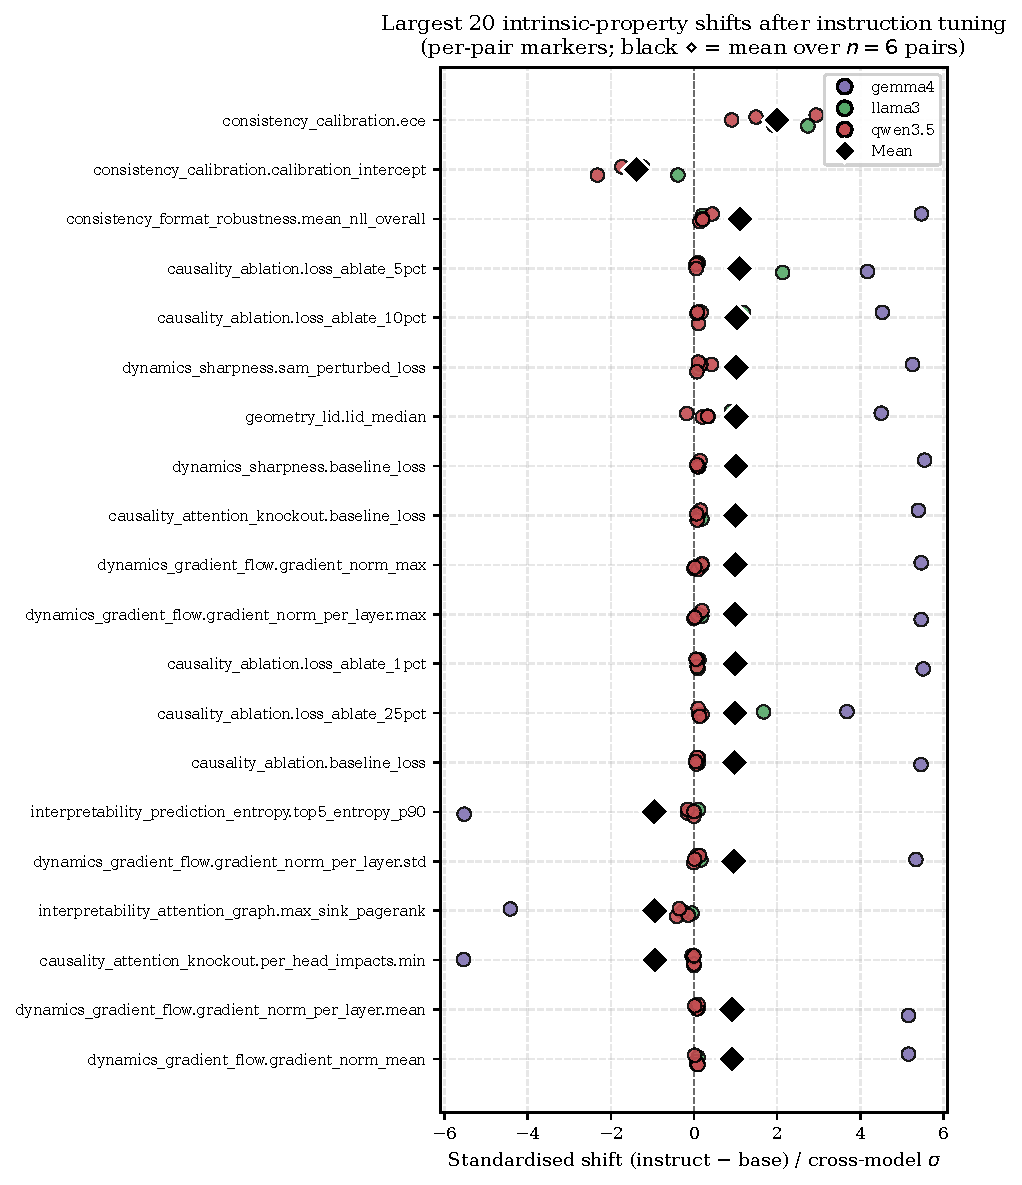
\includegraphics[width=\linewidth]{figures/fig_base_vs_instruct_forest.pdf}
  \caption{Forest plot of the largest base$\to$instruct shifts on the completed BLME pass. Each colored marker is a single base/instruct pair (jittered vertically for readability); the black diamond is the per-feature mean. The dashed vertical line is the no-change baseline. Features are ordered by $|\widetilde{\Delta}|$. Unanimous direction across all six pairs is the primary descriptive evidence at this sample size.}
  \label{fig:bvi-forest}
\end{figure}

% ------------------------------------------------------------
\subsection{Unsupervised Clustering}
\label{sec:clustering}
% ------------------------------------------------------------

We perform PCA on the ($32$ models $\times$ $731$ features) standardised matrix to visualise the intrinsic-property landscape.
The top three components explain $49.5\%$ of total variance ($21.4\%$, $15.6\%$, $12.5\%$).
PC1 aligns strongly with the composite benchmark ($\rho = +0.84$) and moderately with $\log N_{\text{params}}$ ($\rho = +0.60$), suggesting PC1 captures a latent ``capability'' axis that is correlated with but not reducible to scale.
PC2 separates chat-tuned from base models within each family, consistent with the unanimous instruction-tuning shifts reported in \Cref{sec:instruct}.
See \Cref{fig:pca-clustering}.

\begin{figure}[t]
  \centering
  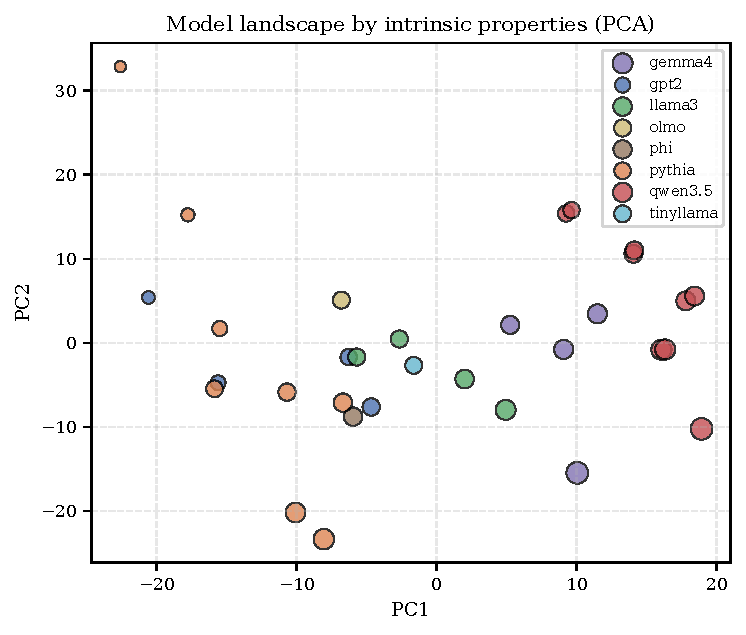
\includegraphics[width=0.8\linewidth]{figures/fig_pca_clustering.pdf}
  \caption{PCA of the $32 \times 731$ intrinsic-feature matrix. Models are colored by family and shaped by base/instruct status. PC$1$--$3$ explain $21.4\%$, $15.6\%$, $12.5\%$ of variance. PC$1$ correlates with composite benchmark ($\rho = +0.84$) and $\log N_{\text{params}}$ ($\rho = +0.60$); PC$2$ separates chat-tuned from base within each family.}
  \label{fig:pca-clustering}
\end{figure}

% ------------------------------------------------------------
\subsection{EDG Evaluation}
\label{sec:edg-eval}
% ------------------------------------------------------------

We evaluate EDG's predictive power through:
(1) Spearman correlation with the composite score;
(2) partial correlation controlling for $\log N_{\text{params}}$;
(3) comparison of $R^2$ against every other individual metric;
(4) within-family analysis in the Pythia series;
(5) paired comparison in base--instruct pairs.

% ------------------------------------------------------------
\subsection{Statistical Power}
\label{sec:power}
% ------------------------------------------------------------

With $n \approx 30$ models, the minimum detectable Spearman correlation at $\alpha = 0.05$ with power $0.8$ is $r \approx 0.45$, corresponding to medium-to-large effects.
We can reliably detect metrics that explain $\gtrsim\!20\%$ of variance.
Within-family results (Pythia $n=8$, GPT-2 $n=4$) have limited power and are reported as exploratory.

% ============================================================
\section{Discussion}
\label{sec:discussion}
% ============================================================

% ------------------------------------------------------------
\subsection{Findings}
% ------------------------------------------------------------

Several predicted patterns from prior work are confirmed in our data.
The spectral exponent $\alpha$ correlates with within-Pythia composite performance at $\rho = -0.88$ on \texttt{median\_alpha} and $-0.83$ on \texttt{std\_alpha}, consistent with Heavy-Tailed Self-Regularization~\citep{martin2021implicit}.
Instruction tuning produces large unanimous shifts in calibration (ECE $+2.0\sigma$, calibration intercept $-1.4\sigma$) consistent with the known RLHF calibration-damage effect, and unanimously sharpens the loss landscape ($+0.99\sigma$ Hutchinson trace and SAM-perturbed loss) supporting the specialisation hypothesis. The effective-rank depth profile, which operationalises information-bottleneck theory, predicts capability beyond scale: \texttt{collapse\_ratio} partial $\rho = +0.68$ and \texttt{erank\_per\_layer.q75} partial $\rho = +0.71$ controlling for $\log N_{\text{params}}$.

Partial correlations will reveal which of these effects survive after controlling for model size.
We expect that some geometric metrics (effective rank utilization, LID) capture aspects of representation quality that size alone does not predict---for instance, two models of similar size but different training recipes may differ substantially in their compression profiles.

% ------------------------------------------------------------
\subsection{Limitations}
% ------------------------------------------------------------

Several limitations deserve emphasis.
First, \textbf{correlation does not imply causation}: observing that a metric correlates with performance does not establish that the measured property causes better performance.
Experimental interventions during training would be needed to establish causal claims.
Second, our sample size ($n = 32$) limits statistical power. A $B = 200$ out-of-bag bootstrap gives a 95\% CI of $[+0.07, +0.90]$ on the held-out LASSO $R^2$ and $[-0.30, +1.03]$ on the gain over the $\log N_{\text{params}}$ baseline. The lower CI bound on the \emph{gain} is below zero, so at $\alpha = 0.05$ our data cannot reject the null that the intrinsic signals add nothing; the median bootstrap gain is $+0.30$, which agrees with the point estimate.
Third, cross-family transfer is data-hungry: the pooled leave-one-family-out $R^2 = 0.27$ masks two opposite regimes — on held-out families with $\geq 8$ models (Pythia, Qwen~3.5) the LASSO materially beats the baseline (MAE reduction of $0.08$--$0.16$), but on single-model families (OLMo, Phi, TinyLlama) the simpler baseline is safer. The intrinsic-metric recipe therefore works best when a new architecture family ships a multi-scale zoo.
Fourth, all evaluations use English text from WikiText-103; intrinsic properties may behave differently for multilingual models evaluated on non-English benchmarks.
Fifth, forward-pass metrics capture a snapshot of trained model behavior and do not reflect training dynamics.
Sixth, several of the strongest size-independent predictors (tokenizer efficiency, vocabulary size, word-tracking) are confounded with training-data volume and tokenizer generation rather than representing pure geometric properties of the trained model.

% ------------------------------------------------------------
\subsection{Implications}
% ------------------------------------------------------------

The $+0.34$ absolute held-out $R^2$ gain from intrinsic signals over $\log N_{\text{params}}$ has concrete implications for multiple audiences.
\textbf{Model developers} can monitor the $26$ LASSO-selected features during training as early indicators of model quality (several are single-forward-pass measurements that cost far less than a full benchmark sweep). In particular the $6$ cross-cited top partial predictors --- RepE task-vector diversity, Ethayarajh word-tracking, LID, weight-activation alignment, Matrix Nuclear-Norm, and massive-activation ratio --- span measurement categories and are therefore not redundant sensors of a single underlying signal.
\textbf{Benchmark designers} can complement behavioral evaluations with these diagnostics to reveal \emph{why} performance varies across architectures. The per-family LOFO breakdown suggests that within a family the cheap diagnostic signals suffice; across families the log-parameter baseline is still a strong default.
\textbf{Theorists} gain empirical grounding for information-bottleneck-style theories: the effective-rank depth profile (\texttt{collapse\_ratio} partial $\rho = +0.68$) carries FDR-significant capability signal beyond $\log N_{\text{params}}$, and the Pedrotti-Guo~2025 compression-valley motif shows up in our data as the dominant cross-architecture erank profile shape.

% ============================================================
\section{Conclusion}
\label{sec:conclusion}
% ============================================================

We have presented a systematic framework for correlating intrinsic model properties with downstream language model performance.
Our metric taxonomy classifies 72 diagnostic measurements by data dependency and model aspect; our normalization framework enables fair comparison across models with different architectures.
A sparse LASSO on the resulting 731 features predicts composite benchmark capability at held-out $R^2 = 0.77$ versus $R^2 = 0.43$ for a $\log N_{\text{params}}$-only baseline, a $+0.34$ absolute improvement from intrinsic signals alone.
After controlling for scale, the strongest predictors are RepE task-vector diversity, contextualized word-tracking, local intrinsic dimensionality, weight-activation alignment, Matrix Nuclear-Norm, and the massive-activation outlier signature --- a genuinely heterogeneous mix of geometry, interpretability, and causality signals rather than a single dominant category.
The effective-rank depth profile (collapse ratio and per-layer quantiles) adds a FDR-significant signal beyond $\log N_{\text{params}}$, operationalizing bottleneck theory for pretrained transformers.
Cross-family transfer remains an open challenge: leave-one-family-out $R^2 = 0.27$ works well when the held-out family has many models and poorly when it has few.
Together with the open-source BLME toolkit (\url{https://github.com/dtsaras/beyond_lm_eval}), this work provides the infrastructure for moving beyond benchmark scores toward understanding the representational foundations of language model capability.

% ============================================================
% Bibliography
% ============================================================
\bibliographystyle{plainnat}
\bibliography{references}

% ============================================================
\newpage
\appendix

% ============================================================
\section{Complete Metric Definitions}
\label{app:metrics}
% ============================================================

This appendix provides the full mathematical definition, hypothesis, and intuition for the 72 diagnostic metrics used as independent variables in our study (the appendix below describes a representative subset; the complete task list is at \url{https://github.com/dtsaras/beyond_lm_eval} in \texttt{src/blme/tasks}). Metrics are organized by category. For each metric we state:
\begin{itemize}
  \item \textbf{Tier}: 1 (weight-only) or 2 (data-dependent, stable).
  \item \textbf{Data requirement}: None, hidden states, attention maps, or interventional (activation patching).
  \item \textbf{Definition}: Full mathematical specification matching our implementation.
  \item \textbf{Hypothesis}: The expected relationship with downstream performance and why.
  \item \textbf{Intuition}: A plain-language explanation of what the metric captures.
  \item \textbf{Normalization}: How the metric is normalized for cross-model comparison.
\end{itemize}

% ============================================================
\subsection{Geometry Metrics}
\label{app:geometry}
% ============================================================

% --------------------------------------------------------
\subsubsection{Weight Spectral Properties (\texttt{geometry\_spectral})}
\label{app:spectral}

\textbf{Tier:} 1 \quad \textbf{Data requirement:} None (weight matrices only)

\textbf{Definition.}
For each linear weight matrix $W \in \mathbb{R}^{m \times n}$ in the model, we compute the singular values $\sigma_1 \geq \sigma_2 \geq \cdots \geq \sigma_{\min(m,n)}$ and derive two quantities:

\emph{Stable rank} measures how spread out the spectrum is relative to the leading singular value:
\begin{equation}
  \text{srank}(W) = \frac{\|W\|_F^2}{\|W\|_2^2} = \frac{\sum_i \sigma_i^2}{\sigma_1^2}
\end{equation}
A stable rank of 1 indicates a rank-1 matrix; a stable rank equal to $\min(m,n)$ indicates a uniform spectrum.

\emph{Power-law exponent} $\alpha$ characterizes the tail behavior of the empirical spectral distribution (ESD). We use the Hill estimator on the top 20\% of singular values:
\begin{equation}
  \hat\alpha = 1 + \frac{k}{\sum_{i=1}^{k} \ln(\sigma_i / \sigma_k)}
\end{equation}
where $k = \lfloor 0.2 \cdot \min(m,n) \rfloor$ and $\sigma_k$ is the $k$-th largest singular value.

We report the mean $\bar\alpha$ and mean stable rank $\overline{\text{srank}}$ across all linear modules.

\textbf{Hypothesis.}
Lower $\alpha$ values (heavier tails) indicate stronger implicit self-regularization and should correlate with better generalization~\citep{martin2021implicit}. Higher stable rank indicates more distributed representations and may also correlate with performance.

\textbf{Intuition.}
The singular value spectrum of weight matrices reflects how the model distributes learned information across its representational capacity. A heavy-tailed spectrum (low $\alpha$) suggests that the model has developed a few very strong features alongside many weaker ones---a hallmark of well-regularized learning. Stable rank measures whether the matrix ``uses'' all its dimensions or concentrates information in a few.

\textbf{Normalization.} Stable rank is already in $[1, \min(m,n)]$ and is comparable across models. $\alpha$ is dimensionless.

% --------------------------------------------------------
\subsubsection{Embedding Hubness (\texttt{geometry\_hubness})}
\label{app:hubness}

\textbf{Tier:} 1 \quad \textbf{Data requirement:} None (embedding matrix only)

\textbf{Definition.}
Given the input embedding matrix $E \in \mathbb{R}^{V \times d}$ where $V$ is vocabulary size, we compute the $k$-nearest-neighbor graph and count how many times each token appears as a neighbor of other tokens. Let $N_k(i)$ denote the number of times token $i$ appears in other tokens' $k$-NN lists. We compute:

\emph{Hubness skewness}: the skewness of the distribution $\{N_k(i)\}_{i=1}^{V}$.

\emph{Hubness Gini coefficient}: the Gini index of the same distribution, measuring inequality.

\emph{Top-1\% mass}: the fraction of all neighbor slots occupied by the top 1\% most frequent hubs.

\textbf{Hypothesis.}
High hubness (positive skewness, high Gini) indicates that a few ``hub'' tokens dominate the nearest-neighbor structure, reflecting anisotropy in the embedding space. Models with lower hubness may have more uniform, isotropic embeddings, which prior work~\citep{cai2021isotropy} associates with better downstream performance.

\textbf{Intuition.}
In high-dimensional spaces, some points become ``universal neighbors''---hubs that are close to almost everything. This curse of dimensionality effect distorts nearest-neighbor structure and can impair the model's ability to discriminate between semantically distinct tokens.

\textbf{Normalization.} Skewness and Gini are dimensionless. No normalization needed.

% --------------------------------------------------------
\subsubsection{Unembedding Structure (\texttt{geometry\_unembedding})}
\label{app:unembedding}

\textbf{Tier:} 1 \quad \textbf{Data requirement:} None (LM head matrix only)

\textbf{Definition.}
We extract the language model head matrix $W_{\text{lm}} \in \mathbb{R}^{V \times d}$ (or its transpose, depending on architecture) and compute:

\emph{Effective rank}: $\text{erank}(W_{\text{lm}}) = \exp\!\bigl(-\sum_i \hat\sigma_i \log \hat\sigma_i\bigr)$ where $\hat\sigma_i = \sigma_i / \sum_j \sigma_j$.

\emph{Weight tying indicator}: whether the model ties input embeddings and output projections ($W_{\text{lm}} = E^T$).

\textbf{Hypothesis.}
The effective rank of the LM head constrains how many ``directions'' the model can use to distinguish tokens in its predictions. Higher effective rank indicates a richer prediction geometry. Weight tying constrains this rank to match the input embedding structure.

\textbf{Intuition.}
The LM head is the final linear map from hidden states to vocabulary logits. If its effective rank is low, the model is effectively making predictions in a low-dimensional subspace regardless of how rich its hidden representations are---a potential bottleneck.

\textbf{Normalization.} Effective rank is divided by $d_{\text{model}}$ for cross-model comparison.

% --------------------------------------------------------
\subsubsection{SVD Isotropy (\texttt{geometry\_svd})}
\label{app:svd}

\textbf{Tier:} 2 \quad \textbf{Data requirement:} Hidden states (last layer)

\textbf{Definition.}
Given the mean-centered hidden-state matrix $X \in \mathbb{R}^{n \times d}$ at the final layer, we compute:

\emph{Effective rank}: $\text{erank}(X) = \exp(H(\hat\sigma))$ as in \Cref{eq:erank}.

\emph{Participation ratio}: $\text{PR}(X) = (\sum_i \sigma_i^2)^2 / \sum_i \sigma_i^4$, which counts the number of ``significantly contributing'' singular values.

\emph{Average cosine similarity}: $\overline{\cos} = \frac{2}{n(n-1)} \sum_{i<j} \cos(x_i, x_j)$, measuring global anisotropy.

\textbf{Hypothesis.}
Higher effective rank and participation ratio indicate more isotropic representations that utilize more of the available dimensions. Lower average cosine similarity indicates less anisotropy. All three should correlate positively with performance~\citep{ethayarajh2019contextual,cai2021isotropy}.

\textbf{Intuition.}
If all hidden states point in roughly the same direction (high cosine similarity, low effective rank), the model wastes most of its representational capacity. Isotropic representations spread information across dimensions, enabling finer-grained discrimination.

\textbf{Normalization.} Effective rank and participation ratio are divided by $d_{\text{model}}$. Cosine similarity is in $[-1, 1]$.

% --------------------------------------------------------
\subsubsection{Local Intrinsic Dimensionality (\texttt{geometry\_lid})}
\label{app:lid}

\textbf{Tier:} 2 \quad \textbf{Data requirement:} Hidden states (last layer)

\textbf{Definition.}
For each query point $x_q$ in the hidden-state matrix, we compute the distances to its $k$ nearest neighbors $d_1 \leq d_2 \leq \cdots \leq d_k$ and estimate the local intrinsic dimensionality using the maximum likelihood estimator~\citep{levina2004maximum}:
\begin{equation}
  \widehat{\text{LID}}(x_q) = -\frac{k}{\sum_{i=1}^{k} \ln(d_i / d_k)}
\end{equation}
We report the mean ($\overline{\text{LID}}$), standard deviation ($\sigma_{\text{LID}}$), median, minimum, and maximum across query points, with $k=20$ by default.

\textbf{Hypothesis.}
LID captures the local dimensionality of the representation manifold around each point. Lower LID relative to $d_{\text{model}}$ indicates that representations lie on a lower-dimensional manifold, suggesting efficient compression. Models that achieve lower LID while maintaining high performance have learned more compact representations.

\textbf{Intuition.}
While effective rank measures global dimensionality, LID measures dimensionality locally---how many directions you can move in from a given point before leaving the data manifold. High variance in LID suggests that different inputs are encoded with different levels of complexity.

\textbf{Normalization.} Divided by $d_{\text{model}}$ to obtain a dimensionality utilization ratio.

% --------------------------------------------------------
\subsubsection{Representation Collapse (\texttt{geometry\_collapse})}
\label{app:collapse}

\textbf{Tier:} 2 \quad \textbf{Data requirement:} Hidden states (all layers)

\textbf{Definition.}
We compute the effective rank at every layer $l \in \{0, 1, \ldots, L-1\}$ using \Cref{eq:erank}, producing a profile $\{\text{erank}(l)\}_{l=0}^{L-1}$.

\emph{Collapse ratio}: $\text{CR} = \text{erank}_{\min} / \text{erank}_{\max}$.

\emph{Maximum drop}: $\Delta_{\max} = \min_l (\text{erank}(l+1) - \text{erank}(l))$, the largest single-layer decrease.

\textbf{Hypothesis.}
A low collapse ratio indicates severe dimensional collapse---the model compresses representations to a small fraction of the available dimensions at some layer. Moderate, smooth collapse (quantified by EDG, \Cref{sec:edg}) should correlate with performance, while extreme or abrupt collapse should not~\citep{jing2021understanding}.

\textbf{Intuition.}
As information flows through layers, some dimensions become inactive. Tracking effective rank across layers reveals whether this compression is gradual (healthy bottleneck) or sudden (potential information loss). The erank profile is also the foundation for our EDG metric.

\textbf{Normalization.} Collapse ratio is in $[0, 1]$. Individual erank values are divided by $d_{\text{model}}$.

% --------------------------------------------------------
\subsubsection{Lipschitz Continuity (\texttt{geometry\_lipschitz})}
\label{app:lipschitz}

\textbf{Tier:} 2 \quad \textbf{Data requirement:} Hidden states (all layers)

\textbf{Definition.}
For each consecutive pair of layers, we compute the relative change in hidden states averaged over all tokens:
\begin{equation}
  L_l = \frac{1}{n}\sum_{i=1}^{n} \frac{\|h_i^{(l+1)} - h_i^{(l)}\|}{\|h_i^{(l)}\| + \epsilon}
\end{equation}
We report the mean ($\bar{L}$) and maximum ($L_{\max}$) across all layer transitions, and the contraction rate (fraction of transitions where $L_l < 1$).

\textbf{Hypothesis.}
The Lipschitz constant controls how much small perturbations in one layer are amplified in the next. Moderate, uniform Lipschitz constants suggest stable information flow. Very high values indicate potential instability; very low values suggest redundant layers.

\textbf{Intuition.}
Each transformer layer applies a residual update $h^{(l+1)} = h^{(l)} + f_l(h^{(l)})$. The Lipschitz ratio measures the magnitude of $f_l$ relative to $h^{(l)}$---whether each layer is making large or small modifications to the representation.

\textbf{Normalization.} Already a ratio; no normalization needed.

% --------------------------------------------------------
\subsubsection{Matrix Entropy (\texttt{geometry\_matrix\_entropy})}
\label{app:matrix-entropy}

\textbf{Tier:} 2 \quad \textbf{Data requirement:} Hidden states (all layers)

\textbf{Definition.}
At each layer $l$, we compute the covariance matrix $\Sigma^{(l)} = \frac{1}{n-1}(X^{(l)})^T X^{(l)}$ of the mean-centered hidden states, obtain its eigenvalues $\lambda_1 \geq \cdots \geq \lambda_d$, normalize them to form a probability distribution $p_i = \lambda_i / \sum_j \lambda_j$, and compute the Von Neumann entropy:
\begin{equation}
  H_{\text{vN}}^{(l)} = -\sum_{i=1}^{d} p_i \log p_i
\end{equation}
We report the mean entropy across layers $\bar{H}_{\text{vN}}$ and the per-layer profile.

\textbf{Hypothesis.}
Higher matrix entropy indicates more uniform eigenvalue distributions---more isotropic covariance structure. Models that maintain high entropy across layers use their representational capacity more efficiently.

\textbf{Intuition.}
Matrix entropy generalizes the notion of effective rank by using the full eigenvalue distribution of the covariance. If a few eigenvalues dominate (low entropy), most variance is captured in a few directions; if eigenvalues are uniform (high entropy), information is spread evenly.

\textbf{Normalization.} Divided by $\log(d_{\text{model}})$ to obtain a fraction of maximum possible entropy.

% --------------------------------------------------------
\subsubsection{Intrinsic Dimension (\texttt{geometry\_intrinsic\_dim})}
\label{app:intrinsic-dim}

\textbf{Tier:} 2 \quad \textbf{Data requirement:} Hidden states (last layer)

\textbf{Definition.}
We use the Two-NN estimator~\citep{facco2017estimating}, which estimates the intrinsic dimension from the ratio of distances to the first and second nearest neighbors. For each point $x_i$, let $r_1(i)$ and $r_2(i)$ be the distances to its nearest and second-nearest neighbor. The intrinsic dimension is:
\begin{equation}
  \hat{d} = \left(\frac{1}{n} \sum_{i=1}^{n} \ln \frac{r_2(i)}{r_1(i)}\right)^{-1}
\end{equation}

\textbf{Hypothesis.}
The Two-NN intrinsic dimension provides a global estimate of the manifold dimension, complementing the local LID estimates. Lower intrinsic dimension relative to $d_{\text{model}}$ indicates more efficient compression.

\textbf{Intuition.}
While LID estimates dimensionality point-by-point, Two-NN gives a single global number answering: ``how many dimensions does the representation manifold actually occupy?'' This is a cruder but more stable measurement.

\textbf{Normalization.} Divided by $d_{\text{model}}$.

% --------------------------------------------------------
\subsubsection{Correlation Dimension (\texttt{geometry\_correlation\_dimension})}
\label{app:corr-dim}

\textbf{Tier:} 2 \quad \textbf{Data requirement:} Hidden states (last layer)

\textbf{Definition.}
The Grassberger--Procaccia estimator~\citep{grassberger1983measuring} computes the correlation integral $C(\epsilon) = \frac{2}{n(n-1)} \sum_{i<j} \mathds{1}[\|x_i - x_j\| < \epsilon]$ and estimates the correlation dimension as the slope of $\log C(\epsilon)$ vs.\ $\log \epsilon$ in the scaling region:
\begin{equation}
  D_2 = \lim_{\epsilon \to 0} \frac{\log C(\epsilon)}{\log \epsilon}
\end{equation}

\textbf{Hypothesis.}
The correlation dimension captures the fractal dimensionality of the representation manifold, which may reveal multi-scale structure not captured by linear methods like effective rank.

\textbf{Intuition.}
Correlation dimension asks: ``if I double the radius of a ball around a point, how does the number of nearby points scale?'' In $d$ dimensions, the count scales as $\epsilon^d$. Fractal (non-integer) dimensions indicate that the data has complex, multi-scale geometric structure.

\textbf{Normalization.} Divided by $d_{\text{model}}$.

% --------------------------------------------------------
\subsubsection{Representational Similarity Analysis (\texttt{geometry\_rsa})}
\label{app:rsa}

\textbf{Tier:} 2 \quad \textbf{Data requirement:} Hidden states (all layers)

\textbf{Definition.}
At each layer $l$, we compute the pairwise distance matrix (representational dissimilarity matrix, RDM) $D^{(l)}_{ij} = \|h_i^{(l)} - h_j^{(l)}\|$ over all pairs of input samples. We then compute the Spearman rank correlation between adjacent layers' RDMs~\citep{kriegeskorte2008representational}:
\begin{equation}
  \text{RSA}(l, l+1) = \rho_S\!\bigl(\text{vec}(D^{(l)}),\; \text{vec}(D^{(l+1)})\bigr)
\end{equation}
We report the mean adjacent RSA ($\bar\rho_{\text{adj}}$) and the early-to-late RSA ($\rho_{\text{early-late}}$).

\textbf{Hypothesis.}
High adjacent RSA indicates that consecutive layers preserve the relative geometry of representations---smooth, gradual transformations. High early-to-late RSA suggests that the model's representational structure remains consistent across depth. Lower early-to-late RSA indicates more transformative processing.

\textbf{Intuition.}
RSA answers: ``do layers agree on which inputs are similar and which are different?'' If adjacent layers have RSA $\approx 1$, the geometry is barely changing; if $\approx 0$, each layer radically reorganizes the representation.

\textbf{Normalization.} Spearman correlation is in $[-1, 1]$; no normalization needed.

% --------------------------------------------------------
\subsubsection{Centered Kernel Alignment (\texttt{geometry\_cka})}
\label{app:cka}

\textbf{Tier:} 2 \quad \textbf{Data requirement:} Hidden states (all layers)

\textbf{Definition.}
CKA~\citep{kornblith2019similarity} measures the similarity between layer representations using kernel alignment. For representations $X \in \mathbb{R}^{n \times p}$ and $Y \in \mathbb{R}^{n \times q}$ (from two layers), linear CKA is:
\begin{equation}
  \text{CKA}(X, Y) = \frac{\|Y^T X\|_F^2}{\|X^T X\|_F \cdot \|Y^T Y\|_F}
\end{equation}
We compute the full $L \times L$ CKA matrix and report the mean adjacent CKA ($\overline{\text{CKA}}_{\text{adj}}$).

\textbf{Hypothesis.}
CKA provides a more principled similarity measure than RSA, being invariant to orthogonal transformations and isotropic scaling. High adjacent CKA throughout the network suggests gradual processing; a block-diagonal CKA matrix reveals phase transitions in representation.

\textbf{Intuition.}
While RSA compares distance patterns, CKA compares the actual linear subspaces used by different layers. Two layers have high CKA if they encode similar information even if individual neuron activations differ.

\textbf{Normalization.} CKA is in $[0, 1]$; no normalization needed.

% --------------------------------------------------------
\subsubsection{HSIC (\texttt{geometry\_hsic})}
\label{app:hsic}

\textbf{Tier:} 2 \quad \textbf{Data requirement:} Hidden states (all layers)

\textbf{Definition.}
The Hilbert--Schmidt Independence Criterion~\citep{gretton2005measuring} measures statistical dependence between layers using kernel methods. For centered kernel matrices $\tilde{K}^{(l)}$ and $\tilde{K}^{(l+1)}$:
\begin{equation}
  \text{HSIC}(l, l+1) = \frac{1}{(n-1)^2} \text{tr}(\tilde{K}^{(l)} \tilde{K}^{(l+1)})
\end{equation}
The compression ratio $\text{HSIC}(0, L-1) / \text{HSIC}(0, 0)$ measures how much of the input information survives to the output.

\textbf{Hypothesis.}
Decreasing HSIC with depth indicates information compression. The compression ratio directly quantifies the information bottleneck.

\textbf{Intuition.}
HSIC measures how much knowing one layer's representations tells you about another's. It is the kernel analogue of mutual information and is equivalent to linear CKA when using linear kernels.

\textbf{Normalization.} Compression ratio is already a ratio in $[0, 1]$.

% --------------------------------------------------------
\subsubsection{Positional Decay (\texttt{geometry\_positional\_decay})}
\label{app:positional-decay}

\textbf{Tier:} 2 \quad \textbf{Data requirement:} Attention maps

\textbf{Definition.}
For each attention head, we compute the Spearman rank correlation between token pair distance $|i - j|$ and the corresponding attention weight $a_{ij}$:
\begin{equation}
  \rho_{\text{pos}} = \rho_S\!\bigl(\{|i-j|\}_{i,j},\; \{a_{ij}\}_{i,j}\bigr)
\end{equation}
We report the mean across all heads $\bar\rho_{\text{pos}}$.

\textbf{Hypothesis.}
A negative correlation indicates that attention decays with distance---the model attends preferentially to nearby tokens. This decay pattern reflects the integrity of positional encoding (especially RoPE). Stronger decay may indicate better local context integration.

\textbf{Intuition.}
Does the model pay more attention to nearby tokens? In models with rotary position embeddings, attention should naturally decay with distance. Deviations from this pattern may indicate that the model has learned to override positional biases for long-range dependencies.

\textbf{Normalization.} Spearman correlation is in $[-1, 1]$; no normalization needed.

% ============================================================
\subsection{Topology Metrics}
\label{app:topology}
% ============================================================

% --------------------------------------------------------
\subsubsection{Persistent Homology (\texttt{topology\_homology})}
\label{app:homology}

\textbf{Tier:} 2 \quad \textbf{Data requirement:} Hidden states (selected layers)

\textbf{Definition.}
We compute the Vietoris--Rips persistent homology~\citep{naitzat2020topology} of mean-pooled sentence representations at early, middle, and late layers. This produces persistence diagrams $\text{Dgm}_{H_k}$ for homological dimensions $k \in \{0, 1\}$:
\begin{itemize}
  \item $H_0$ features: connected components. Each feature has a birth time $b$ and death time $d$; the lifespan $d - b$ indicates how persistent the cluster structure is.
  \item $H_1$ features: loops (1-dimensional holes). Their persistence indicates topological complexity.
\end{itemize}
We report the mean persistence $\bar{p}_{H_0}$, $\bar{p}_{H_1}$, and the number of $H_1$ loops at each layer.

\textbf{Hypothesis.}
As representations are processed through layers, topological complexity should simplify: clusters become more separated ($H_0$ persistence increases or stabilizes) and spurious loops disappear ($H_1$ count decreases). Models that achieve cleaner topological simplification may generalize better.

\textbf{Intuition.}
Persistent homology asks: ``what is the shape of the data?'' At a coarse scale, do representations form clusters? Do they have holes or loops? Tracking these topological features across layers reveals how the model progressively simplifies the geometric structure of its representations.

\textbf{Normalization.} Persistence values depend on the scale of hidden states; we normalize by the mean pairwise distance at each layer.

% --------------------------------------------------------
\subsubsection{Betti Curves (\texttt{topology\_betti\_curve})}
\label{app:betti}

\textbf{Tier:} 2 \quad \textbf{Data requirement:} Hidden states (all layers)

\textbf{Definition.}
The Betti number $\beta_k(\epsilon)$ counts the number of $k$-dimensional topological features alive at filtration scale $\epsilon$. We track $\beta_0$ (connected components) and $\beta_1$ (loops) across layers.

The \emph{simplification ratio} measures how much topological complexity is reduced from early to late layers:
\begin{equation}
  \text{SR} = 1 - \frac{\beta_0^{\text{late}}}{\beta_0^{\text{early}}}
\end{equation}

\textbf{Hypothesis.}
Higher simplification ratio indicates that the network successfully merges initially separate clusters into more coherent structures---a sign of effective representation learning.

\textbf{Intuition.}
Tracking Betti numbers across layers is like watching a sculptor at work: the raw marble (early layers) has complex topology, and the finished sculpture (late layers) has simpler, more structured topology.

\textbf{Normalization.} Simplification ratio is in $[0, 1]$. Raw Betti numbers are compared within-model across layers.

% --------------------------------------------------------
\subsubsection{Persistence Entropy (\texttt{topology\_persistence\_entropy})}
\label{app:persistence-entropy}

\textbf{Tier:} 2 \quad \textbf{Data requirement:} Hidden states (all layers)

\textbf{Definition.}
Given a persistence diagram with lifespans $l_1, l_2, \ldots, l_m$, persistence entropy~\citep{rucco2016characterisation} treats the normalized lifespans as a probability distribution:
\begin{equation}
  \text{PE}_{H_k} = -\sum_{i=1}^{m} \frac{l_i}{\sum_j l_j} \log \frac{l_i}{\sum_j l_j}
\end{equation}
We compute PE for $H_0$ and $H_1$ at each layer and report the simplification ratio of persistence entropy from early to late layers.

\textbf{Hypothesis.}
Decreasing persistence entropy across layers indicates that topological features become more heterogeneous (dominated by a few persistent features) rather than uniformly distributed. This simplification reflects progressive abstraction.

\textbf{Intuition.}
If all topological features have similar lifespans (high entropy), the topology is ``noisy'' with no dominant structure. If a few features have long lifespans and many have short ones (low entropy), the topology is dominated by robust, meaningful structures.

\textbf{Normalization.} PE is in $[0, \log m]$; we normalize by $\log m$ when comparing across layers.

% ============================================================
\subsection{Interpretability Metrics}
\label{app:interpretability}
% ============================================================

% --------------------------------------------------------
\subsubsection{Logit Lens (\texttt{interpretability\_logit\_lens})}
\label{app:logit-lens}

\textbf{Tier:} 2 \quad \textbf{Data requirement:} Hidden states (all layers)

\textbf{Definition.}
At each layer $l$, we project hidden states through the final layer normalization and language model head to obtain intermediate logits, then compute:

\emph{Layer accuracy}: the fraction of tokens for which the argmax of the intermediate logits matches the argmax of the final logits.

\emph{Layer entropy}: the Shannon entropy of the intermediate softmax distribution $H^{(l)} = -\sum_v p_v^{(l)} \log p_v^{(l)}$.

These form a convergence profile showing how predictions crystallize across layers~\citep{nostalgebraist2020logitlens}.

\textbf{Hypothesis.}
Models that converge to their final predictions earlier (high accuracy at earlier layers) have developed a stronger hierarchical prediction pipeline. The slope and onset of the accuracy curve may predict benchmark performance.

\textbf{Intuition.}
The logit lens lets us ``read the model's mind'' at each layer. In well-organized models, a rough prediction emerges early and is progressively refined. In poorly organized ones, the prediction may not stabilize until the very last layers.

\textbf{Normalization.} Layer indices are normalized to depth $[0, 1]$; accuracy is in $[0, 1]$.

% --------------------------------------------------------
\subsubsection{Attention Entropy (\texttt{interpretability\_attention\_entropy})}
\label{app:attn-entropy}

\textbf{Tier:} 2 \quad \textbf{Data requirement:} Attention maps

\textbf{Definition.}
For each attention head $h$ at layer $l$, we compute the Shannon entropy of the attention distribution over the sequence~\citep{clark2019what}:
\begin{equation}
  H_{l,h} = -\sum_{j=1}^{T} a_{ij} \log a_{ij}
\end{equation}
averaged over all query positions $i$ and input samples. We report the mean entropy per layer and the global mean $\bar{H}_{\text{attn}}$.

\textbf{Hypothesis.}
Higher attention entropy indicates broader, less specialized attention patterns. Instruction-tuned models may exhibit higher entropy (attending more broadly) than base models. The relationship with performance is likely non-monotonic: both extremely focused and extremely diffuse attention may be suboptimal.

\textbf{Intuition.}
Entropy measures how ``spread out'' the attention is. An entropy of $\log T$ means uniform attention (the head looks at everything equally); an entropy near 0 means the head focuses on a single token. The distribution of entropies across heads reveals specialization.

\textbf{Normalization.} Entropy is divided by $\log T$ (where $T$ is sequence length) to normalize for different sequence lengths.

% --------------------------------------------------------
\subsubsection{Induction Heads (\texttt{interpretability\_induction\_heads})}
\label{app:induction}

\textbf{Tier:} 2 \quad \textbf{Data requirement:} Attention maps (synthetic repeated tokens)

\textbf{Definition.}
Following \citet{olsson2022context}, we feed the model a sequence with a repeated token pattern $[A] [B] \cdots [A]$ and check whether any attention head at position $[A]_2$ attends strongly to the token following $[A]_1$ (i.e., $[B]$). The induction score for head $(l, h)$ is the attention weight at the correct position.

We report the maximum induction score across all heads ($\max_{\text{ind}}$) and the mean score of the top-$k$ heads ($\bar{s}_{\text{ind}}$).

\textbf{Hypothesis.}
Models with stronger induction heads should exhibit better in-context learning, which may correlate with benchmark performance on tasks requiring pattern matching and few-shot reasoning.

\textbf{Intuition.}
Induction heads implement a simple but powerful algorithm: ``if I've seen token $A$ before, attend to whatever followed $A$ last time.'' This is a building block for in-context learning. Detecting induction heads mechanistically reveals whether the model has learned this fundamental circuit.

\textbf{Normalization.} Induction scores are in $[0, 1]$; no normalization needed.

% --------------------------------------------------------
\subsubsection{Activation Sparsity (\texttt{interpretability\_sparsity})}
\label{app:sparsity}

\textbf{Tier:} 2 \quad \textbf{Data requirement:} Hidden states (MLP activations)

\textbf{Definition.}
After the MLP activation function at each layer, we compute:

\emph{$L_0$ rate}: the fraction of activations above a threshold ($10^{-5}$), measuring the density of the activation pattern.

\emph{Kurtosis}: the fourth standardized moment of activations, measuring heavy-tailedness. High kurtosis indicates that a few neurons fire very strongly while most are near zero.

We report the global mean $L_0$ and kurtosis across all layers.

\textbf{Hypothesis.}
Higher sparsity (lower $L_0$, higher kurtosis) may indicate more efficient feature encoding, where each input activates only a small, specialized subset of neurons. This relates to the superposition hypothesis: sparse activations suggest less superposition.

\textbf{Intuition.}
A sparse MLP activates only a few ``expert'' neurons for each input, while a dense MLP spreads activation broadly. Sparsity reflects whether the model has developed specialized feature detectors or relies on distributed codes.

\textbf{Normalization.} $L_0$ rate is in $[0, 1]$; kurtosis is dimensionless.

% --------------------------------------------------------
\subsubsection{Superposition Index (\texttt{interpretability\_superposition})}
\label{app:superposition}

\textbf{Tier:} 2 \quad \textbf{Data requirement:} Hidden states (MLP activations)

\textbf{Definition.}
For each neuron, we compute the bimodality coefficient of its activation distribution across inputs~\citep{templeton2024scaling}:
\begin{equation}
  \text{BC} = \frac{\gamma^2 + 1}{\kappa}
\end{equation}
where $\gamma$ is skewness and $\kappa$ is kurtosis. A bimodality coefficient $> 5/9$ suggests a bimodal distribution.

\emph{Polysemanticity index}: the mean BC across neurons. Higher values indicate more neurons respond to multiple, distinct input types.

\emph{Neuron utilization rate}: the fraction of neurons with mean activation above a threshold, measuring what fraction of the network is ``active.''

\textbf{Hypothesis.}
Lower polysemanticity (more monosemantic neurons) may indicate cleaner feature representations and better performance. Higher utilization rate suggests more efficient use of model capacity.

\textbf{Intuition.}
In a perfectly monosemantic model, each neuron responds to one concept. In reality, neurons are often polysemantic---responding to multiple unrelated inputs. The superposition index quantifies this: models in ``deep superposition'' pack more features than they have neurons, at the cost of interference.

\textbf{Normalization.} BC and utilization rate are dimensionless.

% --------------------------------------------------------
\subsubsection{Weight--Activation Alignment (\texttt{interpretability\_waa})}
\label{app:waa}

\textbf{Tier:} 2 \quad \textbf{Data requirement:} Hidden states (all layers)

\textbf{Definition.}
At each layer, we compute the top singular vector of the weight matrix ($u_W$, from SVD of the layer's linear projection) and the top principal component of the activation matrix ($u_A$, from PCA of the hidden states). WAA is their absolute cosine similarity:
\begin{equation}
  \text{WAA}^{(l)} = |\cos(u_W^{(l)}, u_A^{(l)})|
\end{equation}
We report the mean $\overline{\text{WAA}}$ across layers.

\textbf{Hypothesis.}
High WAA indicates that the directions most emphasized by the weights align with the directions most used by the activations---the model's capacity matches its usage. Misalignment may indicate wasted capacity or training instability.

\textbf{Intuition.}
If the weight matrix ``wants'' to amplify direction $u_W$ but the actual data primarily varies along a different direction $u_A$, the model is poorly adapted to its inputs. WAA measures this alignment.

\textbf{Normalization.} WAA is in $[0, 1]$; no normalization needed.

% --------------------------------------------------------
\subsubsection{Attention Graph (\texttt{interpretability\_attention\_graph})}
\label{app:attn-graph}

\textbf{Tier:} 2 \quad \textbf{Data requirement:} Attention maps

\textbf{Definition.}
We interpret each attention head's attention matrix as a directed graph (tokens as nodes, attention weights as edges) and compute:

\emph{Sink PageRank}~\citep{xiao2023efficient}: the PageRank centrality of the first token (BOS/CLS), which often acts as an ``attention sink.''

\emph{BOS sink ratio}: the fraction of total attention mass directed to the first token.

\emph{Edge Gini}: the Gini coefficient of attention edge weights, measuring how concentrated attention is among a few token pairs.

\textbf{Hypothesis.}
Strong attention sinks (high BOS PageRank) reflect the model's strategy for handling uninformative attention slots. Edge Gini captures attention sparsity from a graph-theoretic perspective. These structural properties may differ between base and instruction-tuned models.

\textbf{Intuition.}
Viewing attention as a graph reveals global information flow patterns. A model with strong attention sinks ``parks'' attention on a default token when no specific token is relevant---a known phenomenon in efficient inference. The edge Gini reveals whether attention is sparse (a few strong connections) or dense (many weak connections).

\textbf{Normalization.} PageRank is in $[0, 1]$; Gini is in $[0, 1]$.

% ============================================================
\subsection{Causality Metrics}
\label{app:causality}
% ============================================================

% --------------------------------------------------------
\subsubsection{Causal Tracing (\texttt{causality\_tracing})}
\label{app:tracing}

\textbf{Tier:} 2 \quad \textbf{Data requirement:} Interventional (activation patching)

\textbf{Definition.}
Following \citet{meng2022locating}, we perform a three-step procedure:
\begin{enumerate}
  \item \textbf{Clean run}: Record all hidden states and the probability of the target token $p_{\text{clean}}$.
  \item \textbf{Corrupted run}: Add Gaussian noise ($\sigma = 0.1$) to the embedding of subject tokens and record $p_{\text{corrupt}}$.
  \item \textbf{Restored run}: For each layer $l$, patch the clean hidden state back into the corrupted run and record $p_{\text{restore}}^{(l)}$.
\end{enumerate}
The Average Indirect Effect (AIE) at layer $l$ is:
\begin{equation}
  \text{AIE}(l) = \frac{p_{\text{restore}}^{(l)} - p_{\text{corrupt}}}{p_{\text{clean}} - p_{\text{corrupt}}}
\end{equation}
Causal entropy normalizes the AIE distribution across layers into a probability distribution and computes its Shannon entropy, measuring how localized vs.\ distributed the causal effect is.

\textbf{Hypothesis.}
Models with more localized causal effects (low causal entropy, one or few layers with high AIE) have more modular knowledge storage. The location of the maximum AIE (early, middle, or late) may distinguish architectures.

\textbf{Intuition.}
Causal tracing asks: ``if I damage the input and then surgically repair one layer, which repair is most effective?'' This reveals where factual knowledge is stored. A model that stores knowledge in a single layer is more modular than one where knowledge is distributed.

\textbf{Normalization.} AIE is in $[0, 1]$. Layer index is normalized to depth $[0, 1]$.

% --------------------------------------------------------
\subsubsection{Attention Knockout (\texttt{causality\_attention\_knockout})}
\label{app:knockout}

\textbf{Tier:} 2 \quad \textbf{Data requirement:} Interventional (head ablation)

\textbf{Definition.}
For each attention head, we zero out its output and measure the increase in cross-entropy loss relative to the baseline:
\begin{equation}
  \Delta\mathcal{L}_{l,h} = \mathcal{L}_{\text{knockout}(l,h)} - \mathcal{L}_{\text{baseline}}
\end{equation}
We report the maximum knockout impact ($\max \Delta\mathcal{L}$) and the Gini coefficient of the impact distribution.

\textbf{Hypothesis.}
High Gini indicates that a few critical heads dominate model behavior (fragile, specialized architecture). Low Gini suggests a more distributed, redundant architecture. Distributed architectures may be more robust.

\textbf{Intuition.}
By disabling one head at a time and measuring damage, we map the importance landscape. A model where removing any single head barely matters has distributed processing; one where removing a specific head is catastrophic has concentrated, fragile circuits.

\textbf{Normalization.} Gini is in $[0, 1]$; $\Delta\mathcal{L}$ is in loss units (nats or bits).

% ============================================================
\subsection{Representation Engineering Metrics}
\label{app:repe}
% ============================================================

% --------------------------------------------------------
\subsubsection{Task Vectors (\texttt{repe\_task\_vectors})}
\label{app:task-vectors}

\textbf{Tier:} 2 \quad \textbf{Data requirement:} Hidden states (contrastive prompts)

\textbf{Definition.}
Given pairs of prompts with contrasting properties (e.g., positive vs.\ negative sentiment), the task vector at layer $l$ is~\citep{zou2023representation}:
\begin{equation}
  \mathbf{v}^{(l)} = \frac{1}{|\mathcal{P}|}\sum_{(p^+, p^-) \in \mathcal{P}} \bigl(h^{(l)}(p^+) - h^{(l)}(p^-)\bigr)
\end{equation}
We report per-layer norms $\|\mathbf{v}^{(l)}\|$ and cosine similarities between adjacent layers' task vectors.

\textbf{Hypothesis.}
Stronger task vectors (higher norms) indicate cleaner encoding of the target concept. The depth at which task vectors peak may correlate with the model's capability for that task.

\textbf{Intuition.}
A task vector is the ``direction of a concept'' in representation space. If the model cleanly separates positive from negative sentiment, the task vector will be large and consistent. Weak or noisy task vectors suggest the concept is not linearly encoded.

\textbf{Normalization.} Norms are divided by $\sqrt{d_{\text{model}}}$.

% --------------------------------------------------------
\subsubsection{Concept Separability (\texttt{repe\_concept\_separability})}
\label{app:separability}

\textbf{Tier:} 2 \quad \textbf{Data requirement:} Hidden states (contrastive prompts)

\textbf{Definition.}
At each layer, we train a logistic regression classifier (with cross-validation) to distinguish positive from negative examples and report the area under the ROC curve (AUC)~\citep{zou2023representation}:
\begin{equation}
  \text{AUC}^{(l)} = \text{ROC-AUC}\!\bigl(\text{LogReg}(h^{(l)}, y)\bigr)
\end{equation}
We report the per-layer AUC, the maximum AUC across layers ($\max_l \text{AUC}^{(l)}$), and the mean AUC.

\textbf{Hypothesis.}
Higher maximum AUC indicates that the model develops linearly separable concept representations somewhere in its depth. The layer at which separability peaks may relate to the model's processing depth.

\textbf{Intuition.}
If you can train a simple linear classifier to distinguish concepts from hidden states, those concepts are ``linearly readable''---the model has organized its representations so that concept boundaries are flat hyperplanes. This is a stronger claim than having a nonzero task vector.

\textbf{Normalization.} AUC is in $[0.5, 1]$; no normalization needed.

% ============================================================
\section{Model Zoo Details}
\label{app:models}
% ============================================================

\begin{table}[h]
\centering
\caption{Complete model specifications. All models are decoder-only autoregressive transformers with publicly available weights.}
\label{tab:model-details}
\small
\begin{tabular}{@{}llrrrr@{}}
\toprule
\textbf{Model} & \textbf{Family} & $N_{\text{params}}$ & $d_{\text{model}}$ & $L$ & $N_{\text{heads}}$ \\
\midrule
GPT-2 Small & GPT-2 & 124M & 768 & 12 & 12 \\
GPT-2 Medium & GPT-2 & 355M & 1024 & 24 & 16 \\
GPT-2 Large & GPT-2 & 774M & 1280 & 36 & 20 \\
GPT-2 XL & GPT-2 & 1.5B & 1600 & 48 & 25 \\
\midrule
Pythia-70M & Pythia & 70M & 512 & 6 & 8 \\
Pythia-160M & Pythia & 160M & 768 & 12 & 12 \\
Pythia-410M & Pythia & 410M & 1024 & 24 & 16 \\
Pythia-1B & Pythia & 1B & 2048 & 16 & 8 \\
Pythia-1.4B & Pythia & 1.4B & 2048 & 24 & 16 \\
Pythia-2.8B & Pythia & 2.8B & 2560 & 32 & 32 \\
Pythia-6.9B & Pythia & 6.9B & 4096 & 32 & 32 \\
Pythia-12B & Pythia & 12B & 5120 & 36 & 40 \\
\midrule
Llama-3.2-1B & Llama~3 & 1.2B & 2048 & 16 & 32 \\
Llama-3.2-3B & Llama~3 & 3.2B & 3072 & 28 & 24 \\
Llama-3.1-8B & Llama~3 & 8B & 4096 & 32 & 32 \\
\midrule
Qwen-2.5-0.5B & Qwen~2.5 & 0.5B & 896 & 24 & 14 \\
Qwen-2.5-1.5B & Qwen~2.5 & 1.5B & 1536 & 28 & 12 \\
Qwen-2.5-3B & Qwen~2.5 & 3B & 2048 & 36 & 16 \\
Qwen-2.5-7B & Qwen~2.5 & 7B & 3584 & 28 & 28 \\
\bottomrule
\end{tabular}
\end{table}

% ============================================================
\section{Normalization Details}
\label{app:normalization}
% ============================================================

\begin{table}[h]
\centering
\caption{Normalization applied to each metric for cross-model comparability.}
\label{tab:normalization}
\small
\begin{tabular}{@{}lll@{}}
\toprule
\textbf{Metric} & \textbf{Normalization} & \textbf{Range} \\
\midrule
Effective rank (SVD, collapse, unemb.) & $\div\; d_{\text{model}}$ & $[0, 1]$ \\
Participation ratio & $\div\; d_{\text{model}}$ & $[0, 1]$ \\
LID (mean, median) & $\div\; d_{\text{model}}$ & $[0, 1]$ \\
Intrinsic dimension (Two-NN) & $\div\; d_{\text{model}}$ & $[0, 1]$ \\
Correlation dimension & $\div\; d_{\text{model}}$ & $[0, 1]$ \\
Matrix entropy & $\div\; \log(d_{\text{model}})$ & $[0, 1]$ \\
Task vector norms & $\div\; \sqrt{d_{\text{model}}}$ & $[0, \infty)$ \\
\midrule
Stable rank & None (already $[1, \min(m,n)]$) & $[1, \infty)$ \\
Power-law $\alpha$ & None (dimensionless) & $(1, \infty)$ \\
Collapse ratio & None (already a ratio) & $[0, 1]$ \\
Lipschitz constant & None (already a ratio) & $[0, \infty)$ \\
CKA, RSA, WAA & None (correlations) & $[0, 1]$ \\
Attention entropy & $\div\; \log T$ & $[0, 1]$ \\
Sparsity ($L_0$) & None (already a fraction) & $[0, 1]$ \\
Gini coefficients & None (dimensionless) & $[0, 1]$ \\
AUC (separability) & None & $[0.5, 1]$ \\
EDG & None (Spearman $\rho$) & $[-1, 1]$ \\
\bottomrule
\end{tabular}
\end{table}

\end{document}
